This section describes the experiments that uncover the best combination of inputs and epochs as well as the different strategies. Based on the analysis of wind production from Section~\ref{sec:windPowerAnalysis} the network will try to uncover the best approach to predicting the wind power production. Furthermore, experiments are needed to investigate the influence of data manipulation and statistical inputs as presented in Section~\ref{sec:usingStatisticalInput}. Selected test results and graphs can be seen in Appendix~\ref{sec:windResultsAppendix} - relevant results will be shown here. The purpose is to approach the wind power target by attempting different strategies throughout every experiment. Each experiment will either validate or reject its hypotheses and identify what influence wind power production in the Danish electricity market (DK-1). Preferably we see an improvement throughout the experiments.

\todo{DRAWING OF NETWORK}

\subsection{Experiment One - Selection of Input Parameters}
\label{sec:windPowerExperimentOne}
The first experiment is an attempt to find the best constitution of network input parameters based on the analysis in Section~\ref{sec:windPowerAnalysis}. Since the co-relation between wind power and wind speed is significant it will be included as a core input parameter in all test combinations.

\subsubsection{Hypothesis}
The analysis in Section~\ref{sec:windPowerAnalysis} uncovered the co-relation between the different parameters and the wind power production. The following is expected based on the analysis:

\begin{enumerate}
\item Wind speed is expected to be the most influential factor with consumption just behind it. Temperature is expected have the potential to substitute consumption but without achieving as good accuracy. 
\item Air density, time of day, month of year and last known production is expected to be of some influence.
\item Wind direction is expected to be of little influence.
\end{enumerate}

\subsubsection{Variables}
The variables used in this experiment series:

\begin{itemize}
\item Wind speed (WS)
\item Air density (AD)
\item Consumption (C)
\item Time of day (ToD)
\item Temperature (T)
\item Wind direction (WD)
\item Last known production (L-P)
\item Month (Mo)
\item How many percentage of the predictions in the correct direction (\% CD)
\item Neurons in hidden layer 1 (H1)
\item Neurons in hidden layer 2 (H2)
\item Percentage rank from the best prediction (\% Rank)
\end{itemize}

\subsubsection{Basic Input Parameters}
\label{sec:predictionBasicInputParams}
Experiments have been conducted for all possible input combinations. The idea is to discover any unforeseen connection found by the Artificial Neural Network. The results can be found in Appendix~\ref{sec:simpleInputTest} but relevant results will be emphasized here. The results vary in MAE from 127,86 to 199,22. Table~\ref{table:windProdInputParamsTop10} highlight the top and bottom 10 for further analysis. One thing that is not observable from the table is the use of wind speed as the only input for prediction which achieves 149,72 in MAE over the entire year which illustrate the expected relationship between wind speed and wind power. 

The contents of the table further indicates that time of day, air density and last wind power are significant. It correspond well to the analysis in Section~\ref{sec:windPowerAnalysis} where the relationship between wind power and these parameters are established to be of some significance. Last hours wind power is as expected represented in all of top 10 according to the analysis of wind power development in Section~\ref{sec:windProductionDev}. All of the bottom 10 also contains last known wind power but the reason must be found in the inclusion of month. The worst prediction just without month is placed as number three --- the explanation can reside in the size of the training set but this will be discussed later. The inclusion of previous hours will be attempted more sophistically in the experiment about calculated inputs. 

Consumption is only represented five times in top 10 which comes as a surprise due to the correlation established in the analysis of wind power. The consumption showed a close relationship with temperature and the explanation can be a substitution of the two. Air density represents temperature since it is the significant factor in its calculation because due to the pressure being close to constant in the dataset as described in Section~\ref{sec:airDensity}. This is the most plausible explanation of the top-3 being without consumption.

\footnotesize
\begin{center}
\begin{longtable}{|c|c|c|c|c|c|c|c|c|c|c|c|c|}
\hline
\textbf{WS} & \textbf{AD} & \textbf{C} & \textbf{T} & \textbf{WD} & \textbf{L-P} & \textbf{Mo}& \textbf{ToD} & \textbf{MAE} & \textbf{\% Rank} & \textbf{H1} & \textbf{H2} & \textbf{\% CD}  \\
\hline
\endfirsthead
\multicolumn{13}{c}%
{\tablename\ \thetable\ -- \textit{Continued from previous page}} \\
\hline
\textbf{WS} & \textbf{AD} & \textbf{C} & \textbf{T} & \textbf{WD} & \textbf{L-P} & \textbf{Mo}& \textbf{ToD} & \textbf{MAE} & \textbf{\% Rank} & \textbf{H1} & \textbf{H2} & \textbf{\% CD} \\
\hline
\endhead
\hline \multicolumn{13}{r}{\textit{Continued on next page}} \\
\endfoot
\endlastfoot
\arrayrulecolor{light-gray}
 \x &  &  &  \x &  &  \x &  &  \x & 128,32 & 0,0\% & 24 & 1 & 73\% \\ \hline
 \x &  \x &  &  &  \x &  \x &  &  \x & 131,59 & 2,55\% & 17 & 1 & 73\% \\ \hline
 \x &  \x &  &  &  &  \x &  &  \x & 131,89 & 2,78\% & 12 & 1 & 73\% \\ \hline
 \x &  \x &  \x &  \x &  \x &  \x &  &  \x & 133,18 & 3,79\% & 22 & 1 & 72\% \\ \hline
 \x &  \x &  \x &  \x &  \x &  \x &  &  & 133,77 & 4,25\% & 24 & 1 & 73\% \\ \hline
 \x &  \x &  \x &  &  &  \x &  &  \x & 134,14 & 4,54\% & 19 & 1 & 73\% \\ \hline
 \x &  \x &  \x &  &  \x &  \x &  &  \x & 135,4 & 5,52\% & 25 & 1 & 72\% \\ \hline
 \x &  \x &  \x &  &  &  \x &  &  & 136,33 & 6,24\% & 15 & 1 & 73\% \\ \hline
 \x &  \x &  &  &  &  \x &  \x &  \x & 136,65 & 6,49\% & 11 & 1 & 73\% \\ \hline
 \x &  &  &  &  &  \x &  &  & 137,33 & 7,02\% & 1 & 0 & 74\% \\ \hline
 . & . & . & . &  .  & . &  . & . & . & . & . & . & . \\ \hline
 . & . & . & . &  .  & . &  . & . & . & . & . & . & .\\ \hline
 . & . & . & . &  .  & . &  . & . & . & .& . & . & .\\ \hline
 \x &  \x &  &  \x &  &  \x &  \x &  & 170,93 & 33,21\% & 21 & 1 & 71\% \\ \hline
 \x &  &  \x &  \x &  \x &  \x &  \x &  \x & 171,61 & 33,74\% & 23 & 1 & 71\% \\ \hline
 \x &  &  \x &  \x &  &  \x &  \x &  & 172,72 & 34,6\% & 21 & 1 & 71\% \\ \hline
 \x &  &  &  &  \x &  \x &  \x &  & 173,12 & 34,91\% & 17 & 1 & 71\% \\ \hline
 \x &  &  \x &  \x &  &  \x &  \x &  \x & 173,65 & 35,33\% & 12 & 1 & 69\% \\ \hline
 \x &  \x &  \x &  \x &  \x &  \x &  \x &  \x & 174,26 & 35,8\% & 17 & 1 & 68\% \\ \hline
 \x &  \x &  &  \x &  &  \x &  \x &  \x & 174,55 & 36,03\% & 21 & 1 & 71\% \\ \hline
 \x &  &  &  \x &  &  \x &  \x &  \x & 174,85 & 36,26\% & 18 & 1 & 70\% \\ \hline
 \x &  \x &  \x &  &  \x &  \x &  \x &  & 180,89 & 40,97\% & 14 & 1 & 68\% \\ \hline
 \x &  \x &  &  &  \x &  \x &  \x &  \x & 199,22 & 55,25\% & 22 & 1 & 70\% \\ \hline
\caption{Wind Production Input Parameter Test Top and bottom 10. It is based on 3 month of historical data and 200 epochs. It is an average of the prediction over 8000 hours}
\label{table:windProdInputParamsTop10}
\end{longtable}
\end{center}
\normalsize

\noindent The \% CD in Table~\ref{table:windProdInputParamsTop10} is an indication of how many predicted hours was in correct direction compared to the actual direction. The percentage is stable throughout the table with values around 60-70\%. The correct direction percentage is around the same for the bottom 10. It indicates what have been discussed before, namely wind power production follows the trends of the wind speed and it is included in all of the predictions. This will be discussed further when looking at the actual prediction graph.

Wind Direction is represented four times in top 10. What is noticeable is the same combinations without wind direction is also represented. This can suggest the indifference of wind direction, e.g. \#2-\#3 and \#6-\#7 is very similar to each other. This is further backed up by the analysis which only showed a low co-relation.

The contributory cause to the bad accuracy in the bottom is month and how it in general does not help the prediction when using it together with a dataset containing only 3 months. Month represents the seasonal perspective of the input parameters and is suppose to find the relationship between months and the production in general. Since the historical data used for prediction is only 3 months, it does not capture how the same month last year influenced the production. In the case of wind power prediction it seems to be creating more noise and thereby affect the prediction badly. A possible solution to obtain the seasonality aspect is presented in\cite{pjmForecast} where the Neural Network is trained with 45 days from before the day to be predicted, and 45 days before and after in the previous year. By using this approach the month parameter will reflect the influence of the months around you from the last year. This will be validated in an prediction for itself in Section~\ref{sec:predictionWindProdSeasonalExperiment}.

\subsubsection{Importance of testing set}
We describe in our testing procedure that we use a separate training set and a testing set. Table~\ref{table:predictionMAEUnseenVsTrainingSet} emphasize the importance of using a testing set containing only unseen data. The purpose is to generalize beyond the data in the training set and give accurate outputs for unseen data \cite{1} --- the prediction must simulate real use where the training set naturally can't contain known data. It is also noticeable that the MAE is similar from top to bottom. We will only consider the MAE coming from predicting the testing set.

\footnotesize
\begin{center}
\begin{longtable}{|c|c|c|c|}
\hline
\textbf{MAPE (test set)} & \textbf{MAE (test set)} & \textbf{MAE (training set)} & \textbf{MAPE (training set)}  \\
\hline
\endfirsthead
\multicolumn{4}{c}%
{\tablename\ \thetable\ -- \textit{Continued from previous page}} \\
\hline
\textbf{MAPE (test set)} & \textbf{MAE (test set)} & \textbf{MAE (training set)} & \textbf{MAPE (training set)}  \\
\hline
\endhead
\hline \multicolumn{4}{r}{\textit{Continued on next page}} \\
\endfoot
\endlastfoot
\arrayrulecolor{light-gray}
19,34\% & 128,32 & 60,02 & 9,05\%  \\ \hline
19,74\% & 131,59 & 51,54 & 7,73\%  \\ \hline
19,79\% & 131,89 & 51,73 & 7,76\%  \\ \hline
19,98\% & 133,18 & 60,29 & 9,05\%  \\ \hline
20,07\% & 133,77 & 52,17 & 7,83\%  \\ \hline
20,13\% & 134,14 & 54,79 & 8,22\%  \\ \hline
20,32\% & 135,4 & 50,57 & 7,59\%  \\ \hline
20,45\% & 136,33 & 51,69 & 7,76\%  \\ \hline
20,5\% & 136,65 & 53,99 & 8,1\%  \\ \hline
19,76\% & 137,33 & 58,55 & 8,42\%  \\ \hline
 . & . &  . & . \\ \hline 
 . & . &  . & . \\ \hline 
 . & . &  . & . \\ \hline
25,65\% & 170,93 & 51,67 & 7,75\%  \\ \hline
25,75\% & 171,61 & 50,58 & 7,59\%  \\ \hline
25,91\% & 172,72 & 54,5 & 8,18\%  \\ \hline
25,97\% & 173,12 & 53,15 & 7,97\%  \\ \hline
26,05\% & 173,65 & 51,82 & 7,77\%  \\ \hline
26,15\% & 174,26 & 49,84 & 7,48\%  \\ \hline
26,19\% & 174,55 & 54,28 & 8,14\%  \\ \hline
26,23\% & 174,85 & 49,75 & 7,46\%  \\ \hline
27,14\% & 180,89 & 50,92 & 7,64\%  \\ \hline
29,89\% & 199,22 & 52,03 & 7,81\%  \\ \hline
\caption{Average prediction MAE/MAPE on unseen data vs. prediction MAE/MAPE on training set}
\label{table:predictionMAEUnseenVsTrainingSet}
\end{longtable}
\end{center}
\normalsize

\subsubsection{Seasonal aspect}
\label{sec:predictionWindProdSeasonalExperiment}
The discussion above reveals the need for uncovering and discussing how to represent the seasonal aspect (if needed at all) in Artificial Neural Network --- it can be included as a explicit input parameter or implicitly in the dataset by using the right training set size. The training set will be explored with two different sizes in an attempt to express the seasonal aspect:

\begin{enumerate}
\item Basing it on \cite{pjmForecast} where the training set is constructed with 45 days from before the day to be predicted, 45 days before and after in the previous year.
\item Using a year before the day to predict.
\end{enumerate}

The experimental results for (1) are all shown in Appendix~\ref{sec:simpleInputTestSeason} but we will only be focusing on top-10 here because they illustrate the problem. The results are decreased in all of the predictions in Table~\ref{table:seasonalWindProdInputParamsTop10} in comparison with the the results training on 3 months of data. The training set is increased and this might make it harder for the ANN to generalize because too large training sets should according to \cite{1} be avoided due to a tendency to over-train. It can be supported by the similar results only differentiated by 1,12\% from \#1-\#10 --- the network generalizes on much more data and if some values only influence the wind production in smaller periods of the year it will be suffocated between the ones that are important (as with wind speed) over the entire year. The network can over-train itself too much by dedicating to much responsibility to wind speed because it in general is the most important input or it can simply contain too much noise. The possible benefits from including the seasonal aspect when predicting wind power is not enough to make for the loss in accuracy by the increase of training set size, e.g. month is only included once in top-10. Before any final conclusions about the size of training set can be made we will have to conduct the experiment on an entire year.

\footnotesize
\begin{center}
\begin{longtable}{|c|c|c|c|c|c|c|c|c|c|c|c|c|}
\hline
\textbf{WS} & \textbf{AD} & \textbf{C} & \textbf{T} & \textbf{WD} & \textbf{L-P} & \textbf{Mo}& \textbf{ToD} & \textbf{MAE} & \textbf{\% Rank} & \textbf{H1} & \textbf{H2} & \textbf{\% CD} \\
\hline
\endfirsthead
\multicolumn{13}{c}%
{\tablename\ \thetable\ -- \textit{Continued from previous page}} \\
\hline
\textbf{WS} & \textbf{AD} & \textbf{C} & \textbf{T} & \textbf{WD} & \textbf{L-P} & \textbf{Mo}& \textbf{ToD} & \textbf{MAE} & \textbf{\% Rank} & \textbf{H1} & \textbf{H2} & \textbf{\% CD} \\
\hline
\endhead
\hline \multicolumn{13}{r}{\textit{Continued on next page}} \\
\endfoot
\endlastfoot
\arrayrulecolor{light-gray}
 \x &  \x &  \x &  &  \x &  \x &  &  \x & 142,88 & 0,0\% & 7 & 17 & 73\% \\ \hline
 \x &  &  &  \x &  \x &  \x &  &  \x & 142,89 & 0,01\% & 14 & 11 & 73\% \\ \hline
 \x &  \x &  &  &  \x &  \x &  &  \x & 143,37 & 0,34\% & 3 & 21 & 73\% \\ \hline
 \x &  \x &  \x &  \x &  \x &  \x &  &  \x & 143,97 & 0,76\% & 4 & 25 & 72\% \\ \hline
 \x &  &  &  &  &  \x &  &  \x & 143,98 & 0,77\% & 2 & 21 & 72\% \\ \hline
 \x &  \x &  \x &  \x &  &  \x &  \x &  \x & 144,11 & 0,86\% & 1 & 17 & 73\% \\ \hline
 \x &  \x &  &  &  &  \x &  &  \x & 144,12 & 0,87\% & 7 & 12 & 73\% \\ \hline
 \x &  &  &  &  &  &  &  \x & 144,28 & 0,98\% & 12 & 17 & 41\% \\ \hline
 \x &  &  \x &  &  \x &  \x &  &  \x & 144,42 & 1,08\% & 11 & 10 & 72\% \\ \hline
 \x &  \x &  &  \x &  \x &  \x &  &  \x & 144,48 & 1,12\% & 1 & 17 & 73\% \\ \hline
\caption{Top 10 seasonal wind production test. It is based on 3 month of historical data and one month after from the previous year. It is run with 200 epochs and predicts 8000 hours in 2012}
\label{table:seasonalWindProdInputParamsTop10}
\end{longtable}
\end{center}
\normalsize

Table~\ref{table:predictionMAEUnseenVsTrainingSetSeasonality} is included to show MAPE and highlight what discussed regarding the use a testing set with unseen data.

\footnotesize
\begin{center}
\begin{longtable}{|c|c|c|c|}
\hline
\textbf{MAPE (test set)} & \textbf{MAE (test set)} & \textbf{MAE (training set)} & \textbf{MAPE (training set)}  \\
\hline
\endfirsthead
\multicolumn{4}{c}%
{\tablename\ \thetable\ -- \textit{Continued from previous page}} \\
\hline
\textbf{MAPE (test set)} & \textbf{MAE (test set)} & \textbf{MAE (training set)} & \textbf{MAPE (training set)}  \\
\hline
\endhead
\hline \multicolumn{4}{r}{\textit{Continued on next page}} \\
\endfoot
\endlastfoot
\arrayrulecolor{light-gray}
21,44\% & 142,88 & 51.17 & 7.68\% \\ \hline
21,44\% & 142,89 & 50.08 & 7.51\% \\ \hline
21,51\% & 143,37 & 52.01 & 7.8\% \\ \hline
21,6\% & 143,97 & 48.2 & 7.23\% \\ \hline
21,6\% & 143,98 & 49.51 & 7.43\% \\ \hline
21,62\% & 144,11 & 49.31 & 7.4\% \\ \hline
21,62\% & 144,12 & 49.29 & 7.4\% \\ \hline
21,65\% & 144,28 & 121.29 & 18.2\% \\ \hline
21,67\% & 144,42 & 50.5 & 7.58\% \\ \hline
21,68\% & 144,48 & 47.67 & 7.15\% \\ \hline
\caption{Average prediction MAE/MAPE on unseen data vs. prediction MAE/MAPE on training set with seasonality}
\label{table:predictionMAEUnseenVsTrainingSetSeasonality}
\end{longtable}
\end{center}
\normalsize
 
The second experiment where the prediction is based on an entire years training set can be seen in Table~\ref{table:seasonWindProdInputParamsTop2WholeYear}. The MAE is much similar to the first seasonal approach (1) but instead it takes longer time to process because it must train on a larget dataset --- the time aspect will be elaborated in another experiment. Leaving out the seasonal aspect is the obvious choice from the results shown here. Using a training set of 3 months can be argued to contain the seasonal aspect because the set will reflect how the input parameters in general influence the wind power in the current season. Including month or increasing the size of the training set will only add noise and make it harder for the ANN to generalize. The purpose of including month was to avoid problems when encountering a seasonal change due the different conditions from season to season (analysis confirms this). If the same conditions were seen last year then this could be incorporated in the generalization. The results show that the benefits from this approach cannot make up for the small dataset implicitly containing the seasonal aspect. The month parameter will be omitted in experiments to come.   			

\footnotesize
\begin{center}
\begin{longtable}{|c|c|c|c|c|c|c|c|c|c|c|c|c|}
\hline
\textbf{WS} & \textbf{AD} & \textbf{C} & \textbf{T} & \textbf{WD} & \textbf{L-P} & \textbf{Mo}& \textbf{ToD} & \textbf{MAE} & \textbf{MAPE} & \textbf{H1} & \textbf{H2} & \textbf{\% CD}  \\
\hline
\endfirsthead
\multicolumn{13}{c}%
{\tablename\ \thetable\ -- \textit{Continued from previous page}} \\
\hline
\textbf{WS} & \textbf{AD} & \textbf{C} & \textbf{T} & \textbf{WD} & \textbf{L-P} & \textbf{Mo}& \textbf{ToD} & \textbf{MAE} & \textbf{H1} & \textbf{H2} & \textbf{\% CD} \\
\hline
\endhead
\hline \multicolumn{13}{r}{\textit{Continued on next page}} \\
\endfoot
\endlastfoot
\arrayrulecolor{light-gray}
 \x &  \x &  \x &  \x &  &  \x &  \x &  & 147,98 & 22,12\% & 6 & 22 & 73\% \\ \hline
\caption{Seasonal wind production test based on an entire year. It is run with 200 epochs and predicts 8000 hours in 2012}
\label{table:seasonWindProdInputParamsTop2WholeYear}
\end{longtable}
\end{center}
\normalsize

\subsubsection{Best prediction graph}
\label{sec:bestInputCombiGraph}
The first 175 hours of the best prediction from Table~\ref{table:windProdInputParamsTop10} can be seen in Figure~\ref{fig:bestInputParameterPrediction}. The hours have been pointed out because they illustrate situations and issues that are relevant for the analysis and general for the prediction - more graphs can be seen in Appendix~\ref{sec:bestCombiPredictionsGraphs}. It can be observed that the prediction follows the trend of the actual wind production which is also emphasized by the correct direction percentage of 73\%. The graph show how the challenge is the time it takes to identify shifting trends and how much the trend is increasing or decreasing at that particular time. The blue and purple overlay show situations where it is behind the actual trend whereas the yellow overlay illustrates how it is able to identify the rising trend immediate after prediction time (illustrated by the vertical lines) but too early and ends up overshooting. One last comment is in relation to the error visualization in the bottom of the graph and how it follows the curve of the actual wind power productions. MAE is our measure which calculates the difference between the predicted and ideal value and the bigger values will result in bigger MAEs (see section~\ref{sec:maeStatistics} for argumentation for the choice). It points out that we are able to approach small as well as big targets which is also seen from the prediction graph itself.  

\begin{figure}[H]
\centering
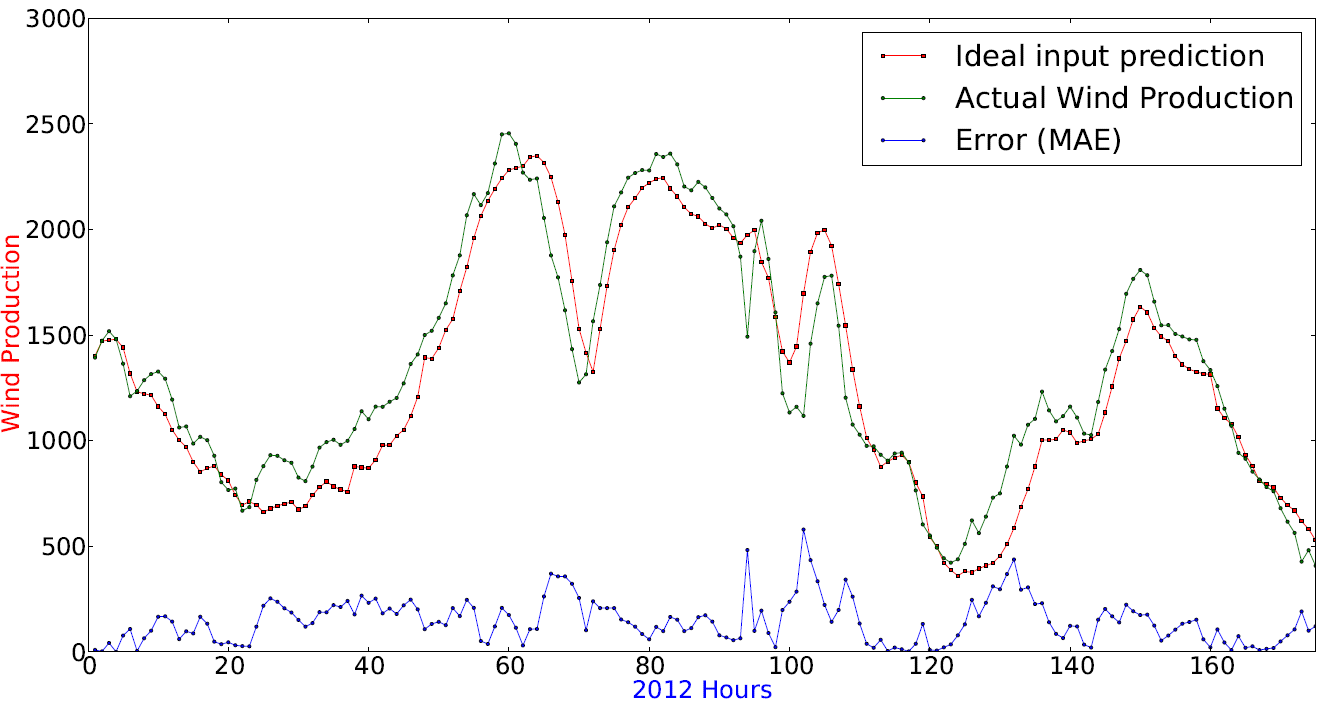
\includegraphics[width=0.99\linewidth]{billeder/bestInputParameterPrediction.png}
\caption{Wind production prediction for 0-175 hours in 2012 with the best combination}
\label{fig:bestInputParameterPrediction}
\end{figure} 

The three overlay situations are emphasized because they show a general problem. Taking a closer look at the purple overlay (hours 120-148) in Figure~\ref{fig:bestInputCombi120-148} illustrates how the prediction is accurate in the beginning but has trouble identifying the significance of the rising trend and continues to under-shoot throughout the entire 24-hours forecast. Every step is based on the prediction from the previous step which is likely to result in a elevated error until a shift in trend.

\begin{figure}[H]
\centering
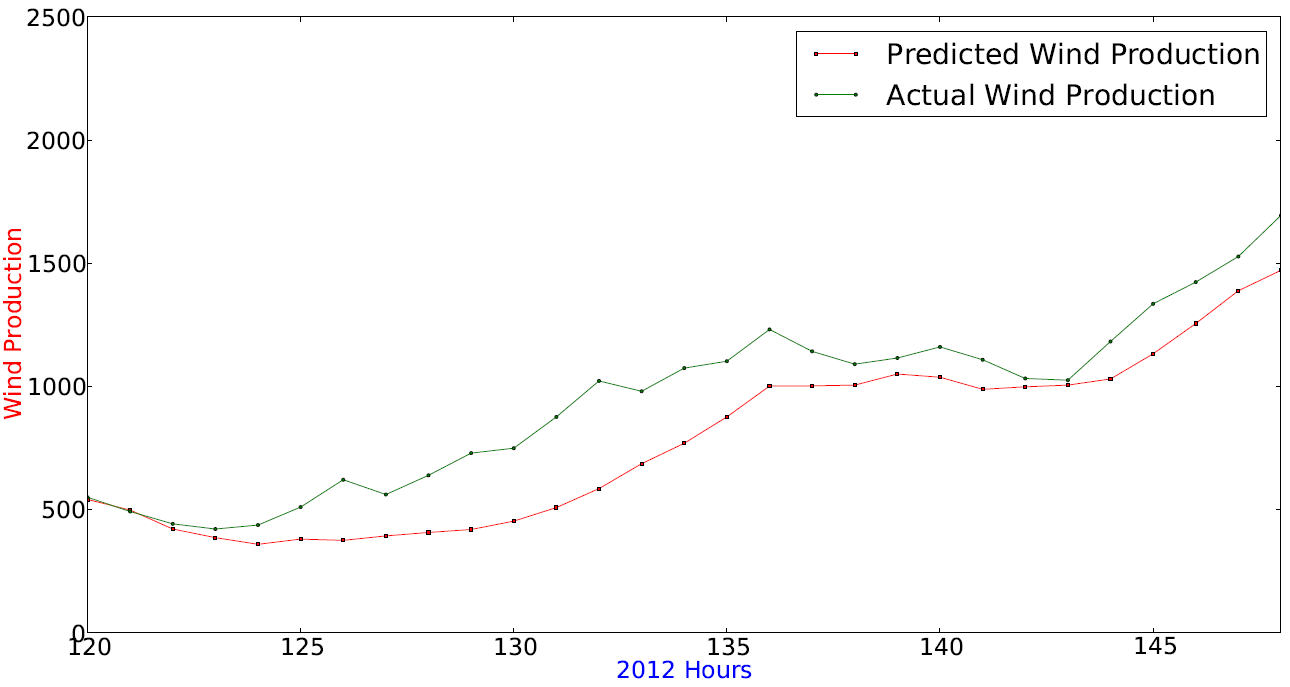
\includegraphics[width=0.99\linewidth]{billeder/bestInputCombi120-148.png}
\caption{Wind production prediction for 24 hours between 120 and 148}
\label{fig:bestInputCombi120-148}
\end{figure} 

The opposite situation with overshooting for the yellow overlay (96-120) is shown in Figure~\ref{fig:bestInputCombi96-120}. It is observable how the prediction again follows accurately in the first couple of hours but then identified the shift too early and overshoots. When the trend shifts again it is able to find its way back, e.g. the error is not elevated from start to end but only per trend. What is meant "per trend" is if the curve is shifting direction and the prediction does not identify it at once it will elevate the error until the trend shifts again. 

\begin{figure}[H]
\centering
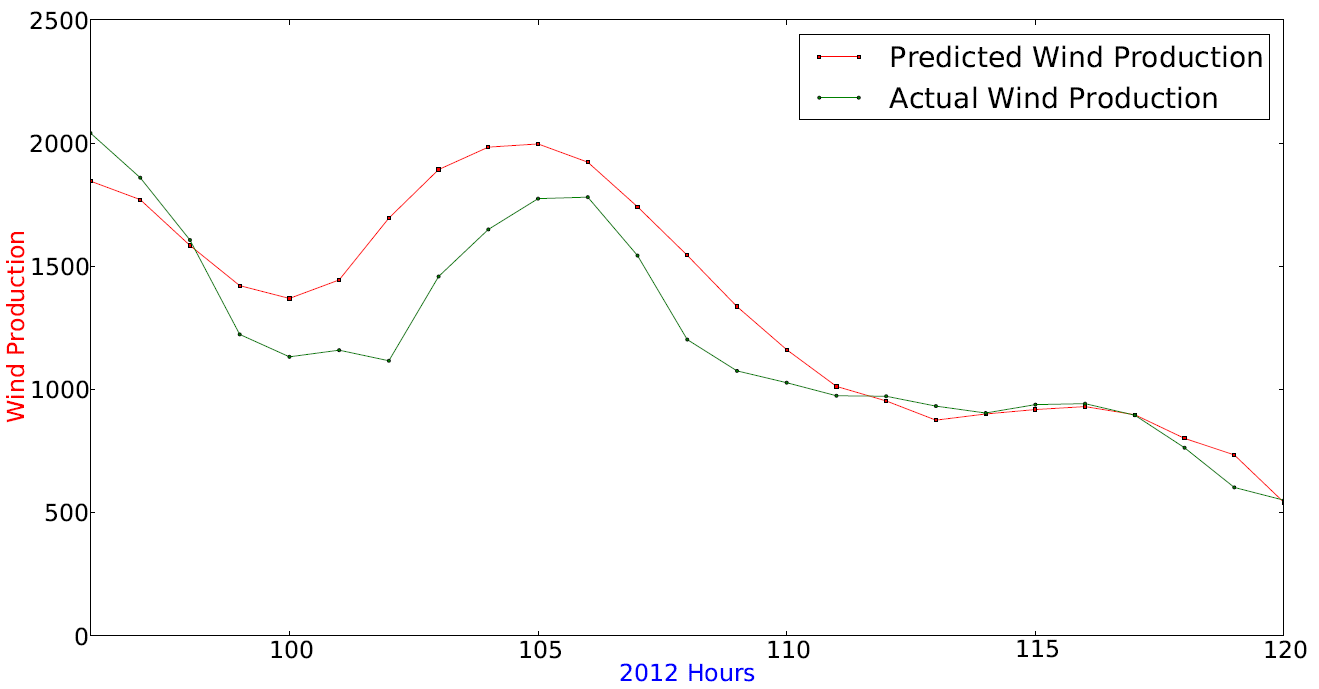
\includegraphics[width=0.99\linewidth]{billeder/bestInputCombi96-120.png}
\caption{Wind production prediction for 24 hours between 96 and 120}
\label{fig:bestInputCombi96-120}
\end{figure} 

What is noticeable from the examples is the problems that arise due to the 24-ahead prediction indicated by the vertical lines. Every hour is based on the previous prediction (except from the first of course) which makes it prone to error if one step fails whilst following a certain direction. It is also obvious that the error is not elevated all the way to the end but only until a new shift in trend is identified --- it can correct itself. The calculated approach described in Section~\ref{sec:usingStatisticalInput} can possible help in these cases by calculating trend or slope and use it as input to add further characteristics of the curve. Experiments will take up this approach for comparison.

The graph in Figure~\ref{fig:bestInputParameterLowNumbers} has been highlighted to show how the best prediction in general performs on low numbers and how it is able to follow the trend all the way from the bottom and up when the wind power is not as volatile (as with the other examples) within the sliding window. High volatility is seen in Figure~\ref{fig:bestInputCombi4500-4700} and again highlights (this time pink) the difficulties in predicting something that is volatile within a short period of time.

\begin{figure}[H]
\centering
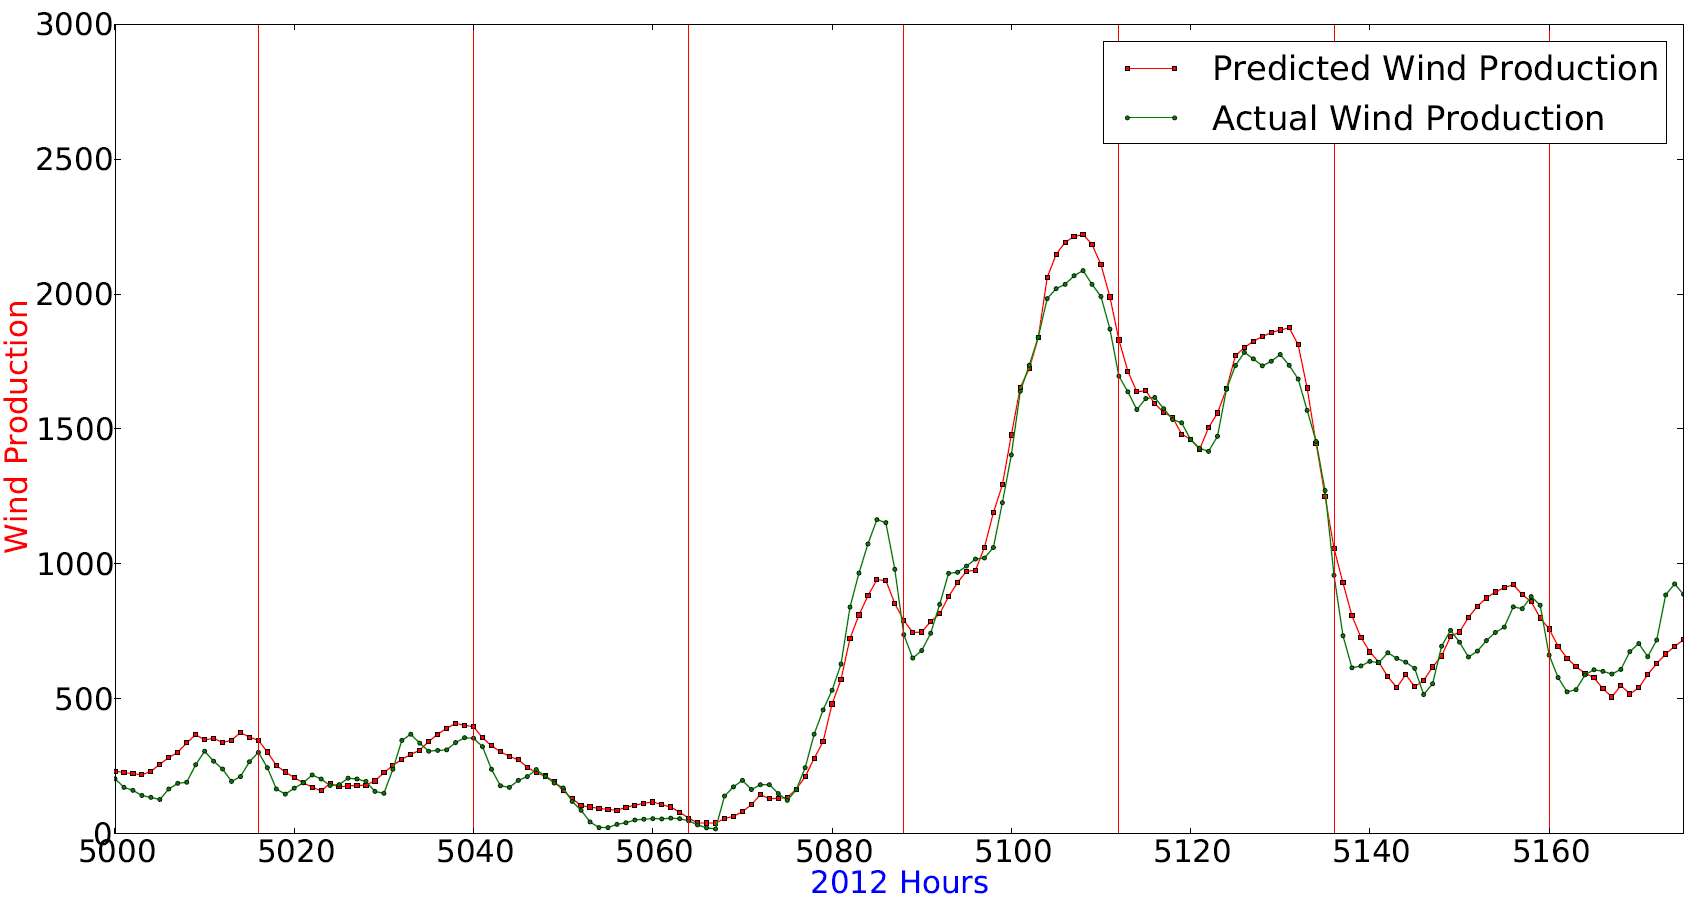
\includegraphics[width=0.99\linewidth]{billeder/bestInputParameterLowNumbers.png}
\caption{Wind production prediction for 5000-5175 hours in 2012 with the best combination}
\label{fig:bestInputParameterLowNumbers}
\end{figure} 

\begin{figure}[H]
\centering
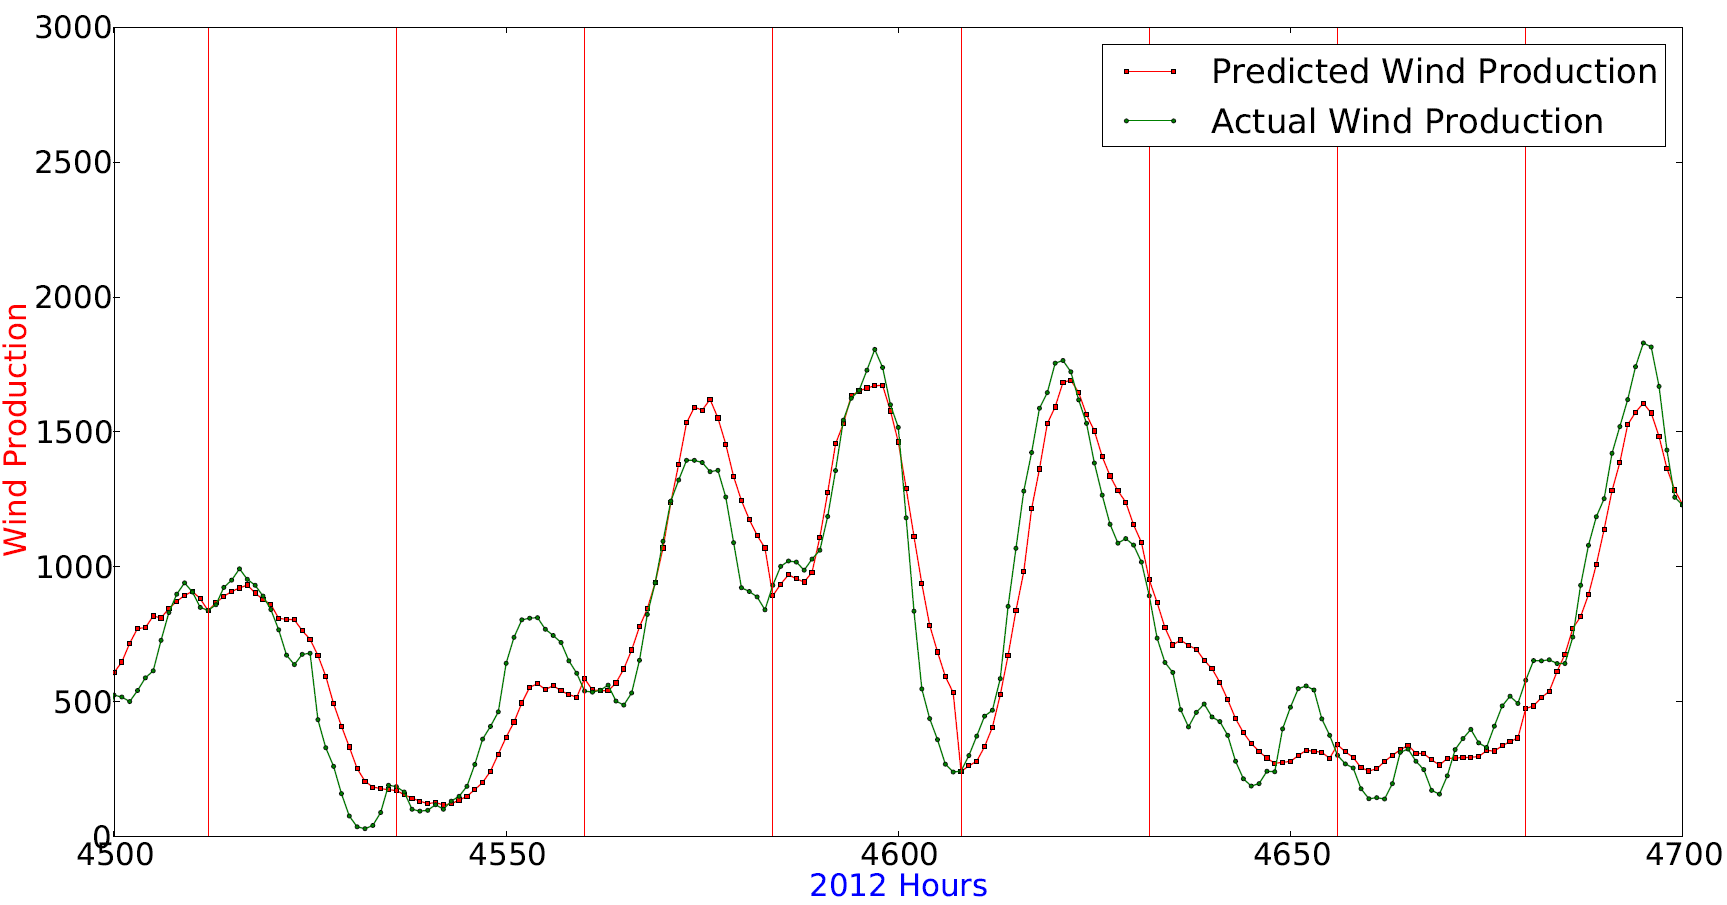
\includegraphics[width=0.99\linewidth]{billeder/bestInputCombi4500-4700.png}
\caption{Wind production prediction for 4500-4700 hours in 2012 with the best combination}
\label{fig:bestInputCombi4500-4700}
\end{figure} 

The correct direction percentage for the best prediction is 73\%. When looking at the graph in Figure~\ref{fig:bestInputCombi4500} some of the obvious wrong directions can be observed in the two pink boxes. When the volatility of the productions are low or less significant then these trends are difficult to identify especially when numbers are smaller as seen Figure~\ref{fig:bestInputParameterLowNumbers} from hours 5000-5060.

\subsubsection{Conclusion}
All results of the first experiment can be seen in Appendix~\ref{sec:windResultsAppendix}. The best result can be seen in Table~\ref{table:windProdInputParamsTop10}. The following conclusions can be made: 

\begin{enumerate}
\item Wind speed showed as expected to have very high significance when predicting the wind power production. Consumption was not represented in top-3 even though it showed very good co-relation in the analysis. The good relationship between temperature and consumption is described in Section~\ref{sec:consumptionWindProduction} which can explain why consumption in top 3 is omitted and substituted with either air density or temperature. The analysis in Section~\ref{sec:airDensity} describes how air density is calculated with temperature as the most significant factor since pressure is close to constant in the dataset.   
\item Last known production is highly represented in both top-10 and bottom-10. It is important when put together with the right combination but whenever in combination with month of year it worsens. Month did not help the prediction even though the dataset was increased to better incorporate the seasonality aspect. Air density and time of day both showed to be highly represented in top-10 and on both on top 3 together with wind speed and last known production.
\item Wind direction was expected little influence bot showed itself four times in top-10. It is assumed that direction is of some importance but not much based on the exact same constitution of input parameters just without wind direction achieved close to same result.
\end{enumerate}

The experiments to come will be based on input combinations from the top 3 from Table~\ref{table:windProdInputParamsTop10}. The inputs are:
\begin{itemize}
\item Wind speed;
\item Air density;
\item Wind Direction;
\item Temperature;
\item Last known production;
\item Time of day;
\end{itemize}
\newpage
\subsection{Experiment Two - Data Manipulation}
\label{sec:windProdExperimentTwo}
Experiment two tries to discover the best way to represent the input data. The need for manipulating the data can arise if irregularities exist that cannot be predicted or simply to adjust the data to better fit the inner workings of the neural network. The 3 approaches to data manipulation tested in the thesis is normalization, trimming and using a matrix as input. The necessity is described in more detail in Section~\ref{sec:DataManipulation}. Normalization is necessary for all input and is used in all experiments because the tanh function is used as activation function. Trimming is used to trim away irregularities if such exist but it does not apply for when predicting wind power production (see Section~\ref{sec:windProductionDev}). It does not leave out the possibility of scenarios where trimming makes sense when used in the hand of an expert, e.g. if experience can eliminate certain high values in the next 24 hours then they could be trimmed. We will investigate whether or not trimming makes the predicted values more accurate in relation to the same values in the predictions without trimming. Tests have been conducted to show the possible benefits from using trimming on wind power production --- both with a trimmed and untrimmed testing set. The purpose of experiment two is to turn inputs into a matrix whenever it makes sense and see the possible benefit of trimming. As described in Section~\ref{sec:Matrix} one input parameter is split into a input parameter for all of its possible values. Each value then has a weight that is adjusted according to the error as illustrated in Section~\ref{sec:annSection}. This is of course only an option if all values are known in advance and of a manageable size. When considering wind production forecasting this is valid for hours of the day, month and wind speed. Only wind speed and time of day will be tested here due to the omitting of the month parameter in experiment one. 

\subsubsection{Hypothesis} 
The matrix manipulation can be applied when values are of a manageable size as discussed in Section~\ref{sec:Matrix}. Based on those discussions the following is expected: 

\begin{enumerate}
\item According to the discussions matrix makes the most sense when values are equally distributed. This apply for time of day and therefore it is expected to see an improvement when matrix is applied here
\item Values are not equally distributed for wind speed and the expectation is instead a worsening in the prediction when applying matrix here.
\end{enumerate}

\subsubsection{Variables}
The variables used in this experiment series:

\begin{itemize}
\item Wind speed (WS).
\item Air density (AD).
\item Time of day (ToD).
\item Time of day as matrix indicated by (m).
\item Temperature (T).
\item Wind direction (WD).
\item Last known production (L-P).
\end{itemize}

\subsubsection{Applying matrix}
The matrix implementation has been applied for wind speed and time of day. The results can be seen in Table~\ref{table:theWindProdInputParamsTop10WithMatrix}. The best results are all without wind speed as matrix and are fairly close to each other. All results with wind speed as matrix are significantly worse and it can already be conclude that wind speed is not applicable for matrix. Wind speeds are represented by 41 different values in our data set which are . Instead of having only one input to represent each of the values, the matrix turned into 41 inputs for every single value. The purpose is to have a weight that tells exactly how much the specific wind speed in general influence the wind production to predict. The network will do so by adjusting a weight for the different wind speeds in the matrix whenever they are seen. As described in Section~\ref{sec:Matrix} a problem arise if some values does not exist or are under-represented. This will cause that specific value to be under-expressed because the weight has only been adjusted a few times or not at all. The seasonal differences in wind power production is described in Section~\ref{sec:windProdSeasonality} and since wind production follows wind speed the training set of only 3 months does not cover all wind speeds. Many wind speed will therefore be under-represented when using wind speed as matrix. 

\begin{center}
\begin{longtable}{|c|c|c|c|c|c|c|c|c|c|c|c|}
\hline
\textbf{WS} & \textbf{AD} & \textbf{C} & \textbf{T} & \textbf{WD} & \textbf{L-P} & \textbf{ToD} & \textbf{MAE} & \textbf{\% Rank} &  \textbf{H1} & \textbf{H2} & \textbf{\% CD}   \\
\hline
\endfirsthead
\multicolumn{12}{c}%
{\tablename\ \thetable\ -- \textit{Continued from previous page}} \\
\hline
\textbf{WS} & \textbf{AD} & \textbf{C} & \textbf{T} & \textbf{WD} & \textbf{L-P} & \textbf{ToD} & \textbf{MAE} & \textbf{\% Rank} &  \textbf{H1} & \textbf{H2} & \textbf{\% CD}  \\
\hline
\endhead
\hline \multicolumn{12}{r}{\textit{Continued on next page}} \\
\endfoot
\endlastfoot
\arrayrulecolor{light-gray}
 \x &  &  &  \x &  &  \x &  \x (m) & 126,25 & 0,0\% & 18 & 17 & 71\% \\ \hline
 \x &  \x &  &  &  &  \x &  \x (m) & 127,95 & 1,35\% & 13 & 19 & 70\% \\ \hline
 \x &  \x &  &  &  \x &  \x & \x (m) & 130,07 & 3,02\% & 2 & 23 & 69\% \\ \hline
 \x (m) & &  &  \x &  &  \x &  \x (m) & 135,71 & 7,49\% & 13 & 16 & 67\% \\ \hline
 \x (m) & \x &  &  &  \x &  \x &  \x & 144,44 & 14,41\% & 14 & 12 & 70\% \\ \hline
  \x (m) & \x &  &  &  &  \x &  \x & 147,63 & 17,12\% & 8 & 16 & 70\%\\ \hline
 \x (m) & \x &  &  &  \x &  \x &  \x (m) & 149,18 & 18,16\% & 13 & 21 & 62\% \\ \hline
 \x (m) & &  &  \x &  &  \x &  \x & 149,19 & 18,17\% & 10 & 22 & 63\% \\ \hline
 \x (m) & \x &  &  &  &  \x &  \x (m) & 155,46 & 23,14\% & 16 & 13 & 59\% \\ \hline
\caption{Matrix test}
\label{table:theWindProdInputParamsTop10WithMatrix}
\end{longtable}
\end{center}

 The significance of time of day is seen in Section~\ref{sec:greenTOD} and the improvement was expected to be somewhat higher since the matrix should make it more expressive. The section shows how the average wind power varies from 750 during the night to around 925 during the day for an entire year. This is not a significant change and because we only train on 3 months of data this difference can be even smaller and therefore the one parameter can express it almost as good as the matrix implementation --- the reason is that all weights in the matrix is adjusted similarly to the one weight when using only one value to represent time of day. If the difference between night and day was more significant it would create more potential for accuracy due to the nature of the matrix. The matrix implementation records individual influences of all of its values so they do not influence each other and thereby letting --- this makes the most sense when there is a big difference between the values so that they do not affect each other badly which. This scenario is illustrated in the analysis of price in Section~\ref{sec:seasonality} where Figure~\ref{fig:price_over_weekdays} shows a 42,4\% difference between the minimum price hour to the maximum price hour. The expectation is to see a better improvement when applying matrix to price than wind power because of this. 

Table~\ref{table:maeAndMAPEForMatrix} shows both MAE and MAPE for the results obtained here. The best result without wind speed as matrix and with time of day as matrix is the same as in Table~\ref{table:windProdInputParamsTop10} but number \#2 and \#3 has switched places but the difference between them is still not significant. Top-3 improved with a total average of 1,9\%.

\begin{center}
\begin{longtable}{|c|c|}
\hline
\textbf{MAPE} & \textbf{MAE} \\
\hline
\endfirsthead
\multicolumn{2}{c}%
{\tablename\ \thetable\ -- \textit{Continued from previous page}} \\
\hline
\textbf{MAPE} & \textbf{MAE} \\
\hline
\endhead
\hline \multicolumn{2}{r}{\textit{Continued on next page}} \\
\endfoot
\endlastfoot
\arrayrulecolor{light-gray}
18,94\% & 126,25 \\ \hline
19,3\% & 127,95\\ \hline
19,52\% & 130,07 \\ \hline
20,36\% & 135,71\\ \hline
21,67\% & 144,44\\ \hline
22,15\% & 147,63 \\ \hline
22,38\% & 149,18\\ \hline
22,38\% & 149,19 \\ \hline
23,32\% & 155,46 \\ \hline
\caption{Graph showing MAE and MAPE for the matrix results}
\label{table:maeAndMAPEForMatrix}
\end{longtable}
\end{center}

\subsubsection{Prediction - Trimming}
The need for trimming exists if irregularities exist or you want to narrow the narrow down the dataset and focus the prediction. In wind power production such values do not exist in our dataset and at the same we want to predict all values over the entire year. This does leave out the possibility that trimming could make the prediction more accurate on certain values outside of the trimmed values. This statement disproved in the context of wind power in Table~\ref{table:trimmingOnBothSetsTable} where all types of trim results in a worsening in MAE. This indicates that values that are necessary for the generalization function to approach its target are removed during trimming. What can be seen though is that the more trim the better the MAE becomes --- this is not necessarily a good sign since bigger values contribute to a bigger MAE.

\begin{center}
\begin{longtable}{|c|c|c|c|c|c|c|}
\hline
\textbf{Trim \%} & \textbf{MAPE}  & \textbf{MAE} & \textbf{\% Rank} & \textbf{Min trim} & \textbf{Max trim} & \textbf{\% CD} \\
\hline
\endfirsthead
\multicolumn{7}{c}%
{\tablename\ \thetable\ -- \textit{Continued from previous page}} \\
\hline
\textbf{Trim \%} & \textbf{MAPE} & \textbf{MAE} & \textbf{\% Rank} & \textbf{Min trim} & \textbf{Max trim} & \textbf{\% CD} \\
\hline
\endhead
\hline \multicolumn{7}{r}{\textit{Continued on next page}} \\
\endfoot
\endlastfoot
\arrayrulecolor{light-gray}
5\% & 19,21\% & 128,91 & 0,0\% & 40 & 2018 & 69\% \\ \hline  
4\% & 19,73\% &  130,94 & 1,57\% & 14 & 2076 & 73\% \\ \hline  
3\% & 20,5\% & 134,19 & 4,1\% & 49 & 2154 & 72\%\\ \hline 
2\% & 20,96\% & 136,27 & 5,71\% & 23 & 2270 & 72\% \\ \hline  
1\% & 20,92\% &  138,19 & 7,2\% & 31 & 2416 & 72\%\\ \hline 
\caption{Trimming from 1\% to 5\%}
\label{table:trimmingOnBothSetsTable}
\end{longtable}
\end{center}
\todo{make it}

Section~\ref{sec:windProductionDev} discuss how trimming would affect the dataset and it is clear that when values are removed it cuts directly in a curve. It results in the possibility of actually creating irregularities instead of removing them. This confirmed by comparing the graph in Figure~\ref{fig:fivePercentTrimPrediction} (with trimming) with the one in Figure~\ref{fig:bestInputPredictFrom0-400} (without trimming). The curves are not as smooth with trimming applied which is apparent when looking at the hours from 48-82 in both graphs. The one without trimming shows how the graph looked before trimming and it is clear the by applying trimming the graph has become more volatile and thereby harder to predict.

\begin{figure}[H]
\centering
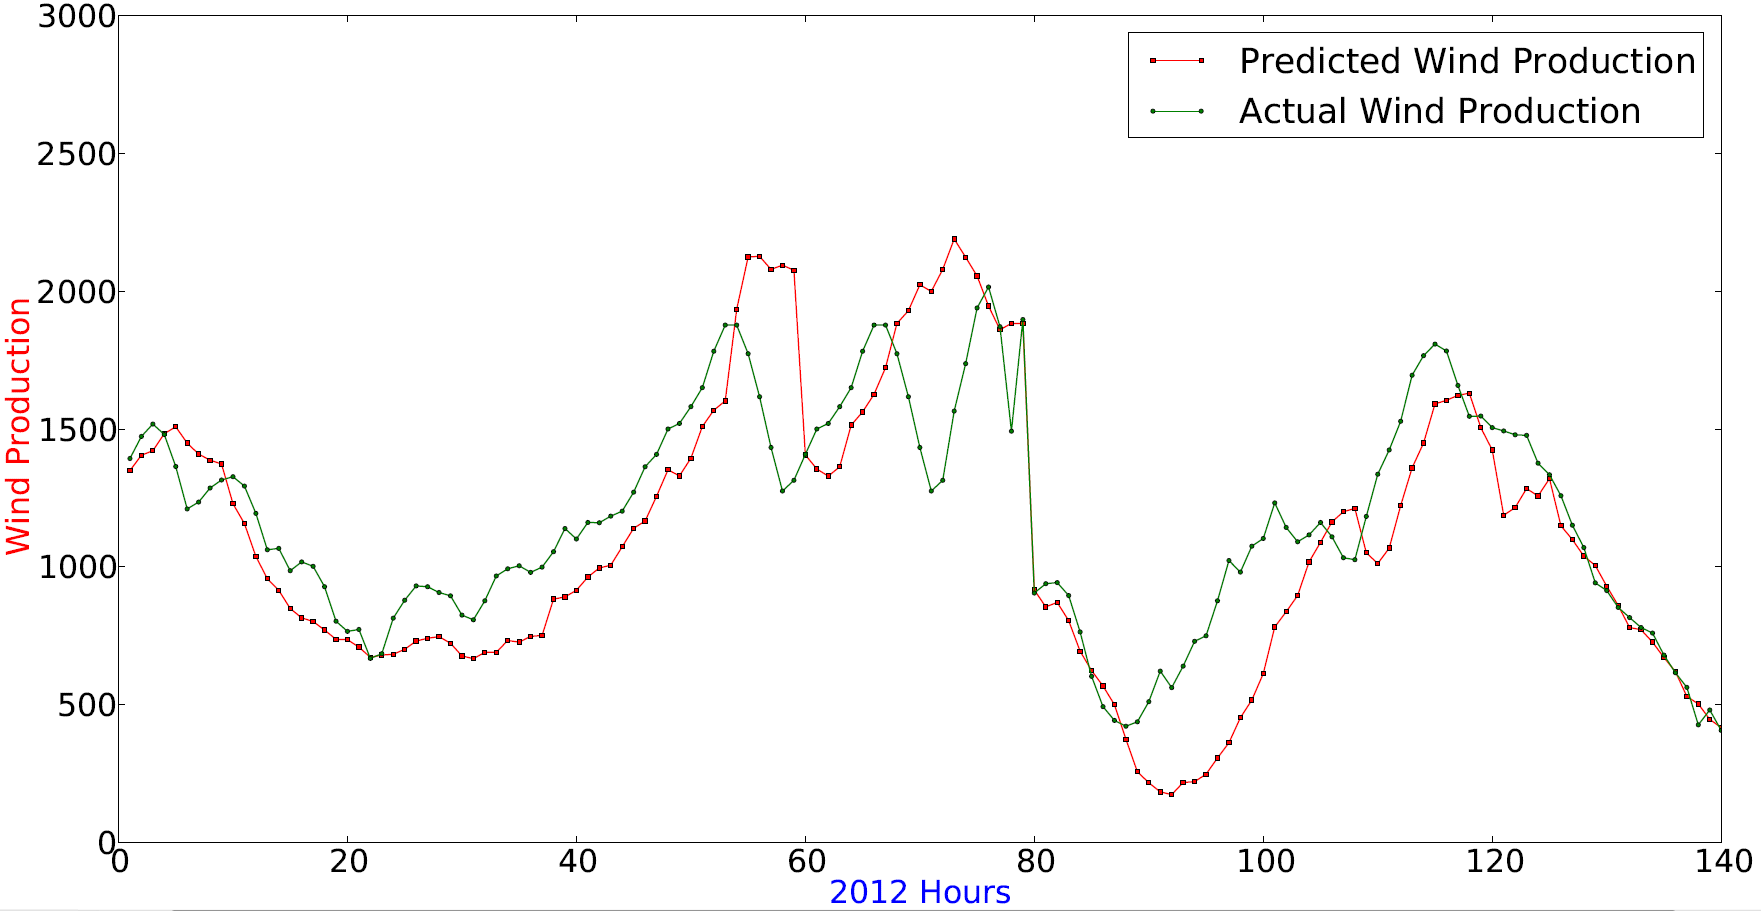
\includegraphics[width=0.99\linewidth]{billeder/fivePercentTrimPrediction.png}
\caption{Wind power prediction for hours 0-400 with 5\% trim}
\label{fig:fivePercentTrimPrediction}
\end{figure} 

\begin{figure}[H]
\centering
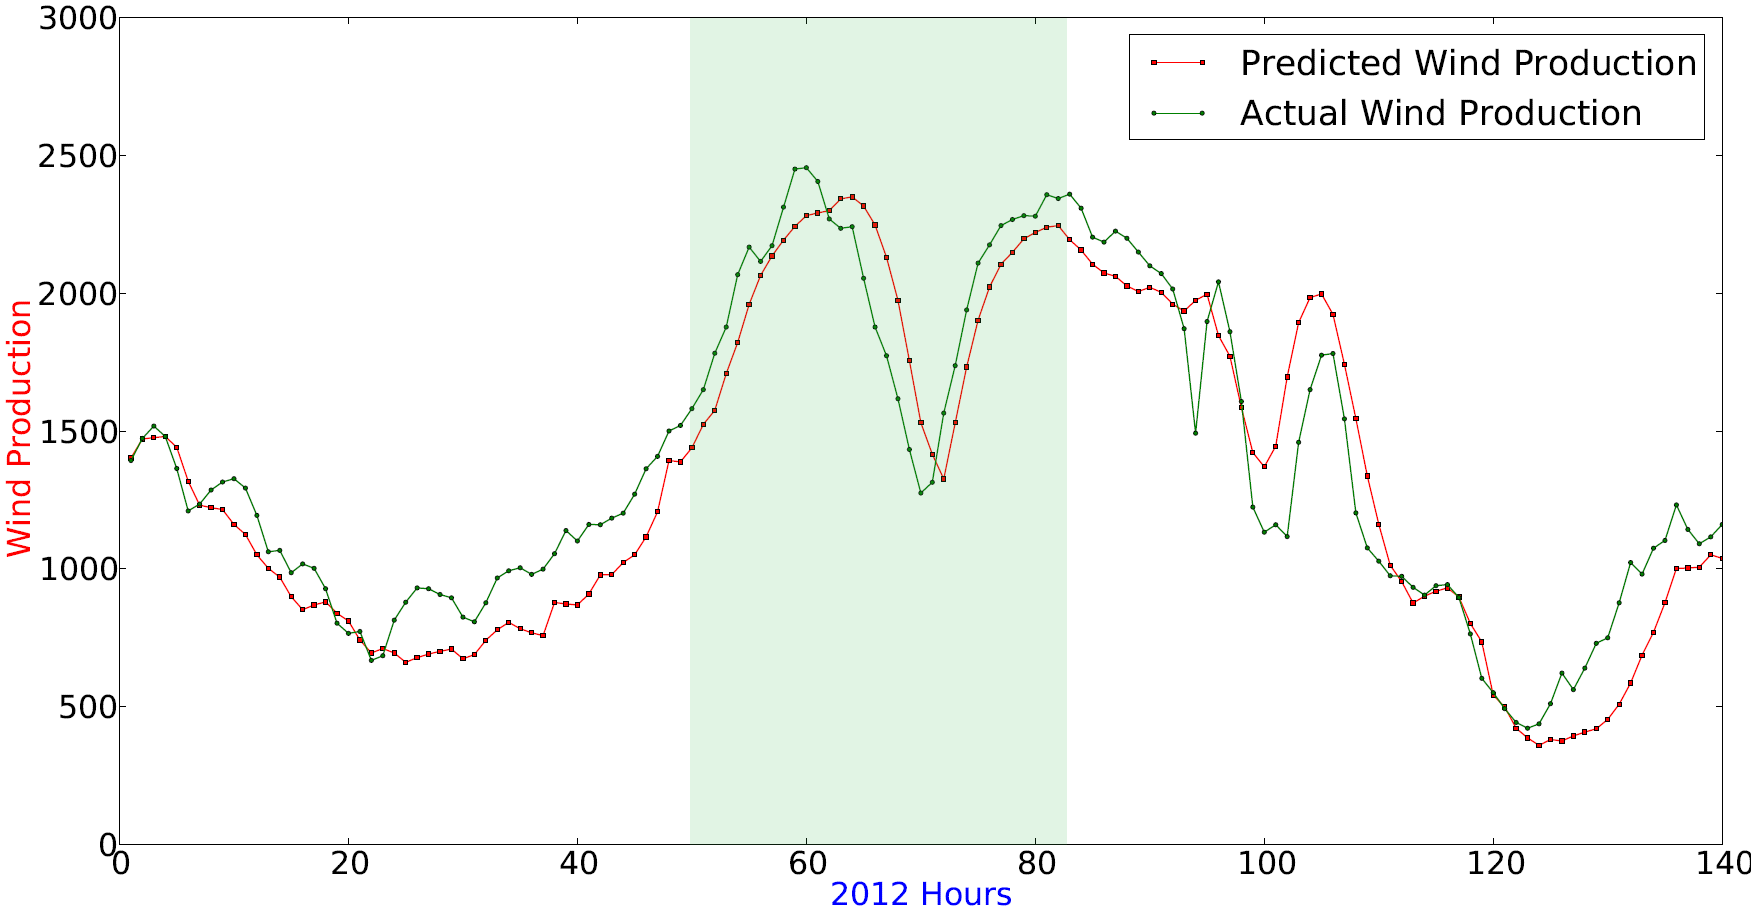
\includegraphics[width=0.99\linewidth]{billeder/bestInputPredictFrom0-400.png}
\caption{Wind power prediction for hours 0-400 with best input combination}
\label{fig:bestInputPredictFrom0-400}
\end{figure} 

\subsubsection{Best prediction graph}
The prediction in Figure~\ref{fig:bestMatrixGraph} is much similar to what was seen in the best prediction from experiment one which is also indicated by the small difference in error. See Section~\ref{sec:bestInputCombiGraph}. 

\begin{figure}[H]
\centering
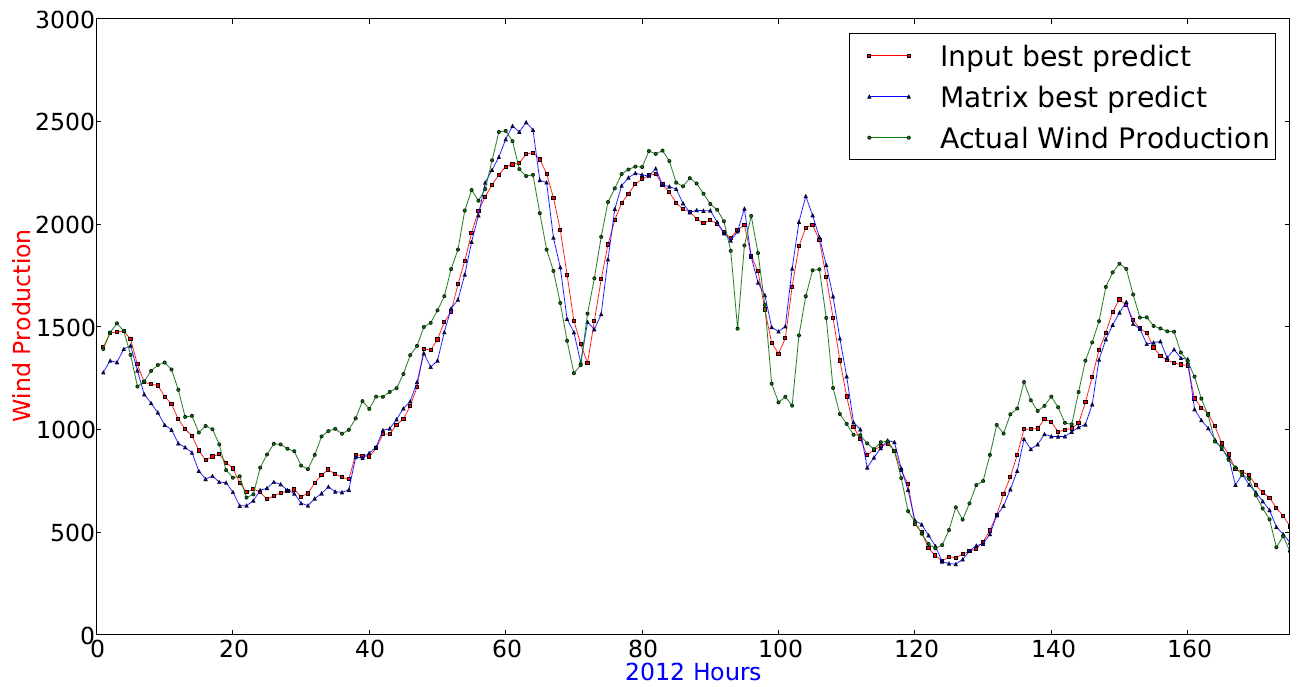
\includegraphics[width=0.99\linewidth]{billeder/bestMatrixGraph.png}
\caption{Wind power prediction for 175 hours in 2012 for the best matrix experiment}
\label{fig:bestMatrixGraph}
\end{figure}   

\subsubsection{Conclusion}
Matrix has been applied to time of day and wind speed. Experiments have been conducted to find where matrix is best applicable.

\begin{enumerate}
\item When applying matrix to time of day there is a slight improvement and it outperformed all predictions with wind speed as matrix. The time of day with matrix predictions are all better than their corresponding prediction in Table~\ref{table:windProdInputParamsTop10}. The improvement is in average only 1,9\% in MAE which is not as significant as expected and it can therefore be argued if matrix is worth the enlargement in input parameters when predicting wind power production. Trade-offs must be made in relation to the time to process and the achieved improvement. The trade-off between time and inputs will be discussed further in a later experiment 
\item The decrease in performance when applying matrix to wind speed can be seen from the results in Table~\ref{table:theWindProdInputParamsTop10WithMatrix}. The decrease can be due to the wind speed values not being equally distributed and therefore in some cases be under-represented and not able to be expressed properly.  
\end{enumerate}

The improvement by applying matrix to time of day is considered enough for next experiment under the circumstances of our test procedure from Section~\ref{sec:testProcedure}. Wind speed as matrix will be omitted.

\newpage

\subsection{Experiment Three - Calculated Inputs}
The experiments here will be focusing on the concepts described in Section~\ref{sec:usingStatisticalInput}. The importance of the current wind production development is described in Section~\ref{sec:windProductionDev} and it describes how the wind production has high volatility and follow certain tendencies. The purpose is to add inputs that in some way analyse productions from immediate past hours to help the existing generalization approach its target more accurately in a specific hour. We therefore see it as independent from the input analysis since it will help the best of the input combinations to perform better. All of the approaches take outset in previous hours so the first step is to find the best number of previous hours to calculate upon. Secondly, they must be tested in combination with each other to find the best combination. The different approaches are historical volatility, skewness, simple, slope calculation and inclusion of previous productions as input. 

\subsubsection{Hypothesis} 
It is the hypothesis that the different approaches will help the neural network approach its target better by adding knowledge about the current trend for every hour. It leads to: 

\begin{enumerate}
\item Wind production is volatile and therefore it is expected that the historical volatility will help the generalization to approach its target.
\item Section~\ref{sec:windProductionDev} explains the need for identifying the development of the curve. Beside from historical volatility it comes in 3 different approaches: 1) skewness; 2) slope calculation and 3) previous productions as input. The expectation is to see a slight increase in performance when these are applied.
\item It is the expectation to achieve better accuracy when combining the different approaches.
\end{enumerate}

\subsubsection{Variables}
The variables used in this experiment series:

\begin{itemize}
\item Wind speed (WS).
\item Air density (AD).
\item Time of day as matrix (ToD).
\item Temperature (T).
\item Wind direction (WD).
\item Last known production (L-P).
\item Historical volatility (V).
\item Skewness (S).
\item Simple slope calculation (C).
\item Previous productions as input (Scatter/Sc)
\end{itemize}

\subsubsection{Historical Volatility}
\label{sec:predictionHistVol}
Historical Volatility is presented in Section~\ref{sec:usingStatisticalInput}. The purpose is to calculate the historical volatility for one hour based on a predefined number of previous hours, e.g. every hour in the training set will calculate the historical volatility from for instance 20 hours just before it (except from the first 20 hours). The volatility calculation will be based on EWMA from Section~\ref{sec:ewmaVolatility} which requires a smoothing factor between 0-1 that needs to be found through experiments. The experiment has been conducted for smoothing factors between 0,1 and 0,9 on hours between 4-24. The best established rate with the best number of hours for the dataset is tested on top-3 from Table~\ref{table:theWindProdInputParamsTop10WithMatrix}.

\footnotesize
\begin{center}
\begin{longtable}{|c|c|c|c|c|c|}
\hline
\textbf{Previous Hours} & \textbf{Smoothing factor}& \textbf{MAPE} & \textbf{MAE} & \textbf{\% Deviation} & \textbf{\% CD} \\
\hline
\endfirsthead
\multicolumn{6}{c}%
{\tablename\ \thetable\ -- \textit{Continued from previous page}} \\
\hline
\textbf{Previous Hours} & \textbf{Smoothing factor}& \textbf{MAPE} & \textbf{MAE} & \textbf{\% Deviation} & \textbf{\% CD} \\
\hline
\endhead
\hline \multicolumn{6}{r}{\textit{Continued on next page}} \\
\endfoot
\endlastfoot
\arrayrulecolor{light-gray}
6 & 0,70 & 18,28\% & 121,81 & 0,0\% & 73\% \\ \hline
20 & 0,80 & 18,44\% & 122,9 & 0,89\% & 70\%  \\ \hline
24 & 0,60 & 18,47\% & 123,13 & 1,08\% & 71\& \\ \hline
24 & 0,80 & 18,61\% & 124,02 & 1,81\% & 70\% \\ \hline
16 & 0,20 & 18,85\% & 125,65 & 3,15\% & 69\% \\ \hline
12 & 0,30 & 19,05\% & 127,0 & 4,26\% & 70\% \\ \hline
24 & 0,70 & 19,06\% & 127,06 & 4,31\% & 69\% \\ \hline
16 & 0,60 & 19,11\% & 127,38 & 4,57\% & 69\% \\ \hline
24 & 0,40 & 19,13\% & 127,51 & 4,68\% & 70\% \\ \hline
16 & 0,90 & 19,17\% & 127,77 & 4,89\% & 69\% \\ \hline
\caption{Historical volatility on different hours and with different smoothing factors}
\end{longtable}
\label{table:historicalVoltalityHours}
\end{center}
\normalsize

All combinations of smoothing factor and previous hours can be seen in Appendix~\ref{sec:historicalVolatiltiyResultsAppendix} --- only top 10 is shown here. The results in Table~\ref{table:historicalVoltalityHours} show that a smoothing factor of 0,70 calculated on the 6 previous hours is the best choice. The expectation was to get a low smoothing factor due to the fluctuations in the wind power production as described in Section~\ref{sec:ewmaVolatility}. The reason for the higher factor can be explained with the number of previous hours being too small to reflect the many changes, e.g. if the historical volatility was calculated over the entire dataset it would probably be smaller. We can see from the graph in Figure~\ref{fig:bestVolatilityVsMatrixGraph} that the curves are much similar to the curves without volatility which is expected since the volatility approach is an augmentation of the best prediction with matrix. 

\begin{figure}[H]
\centering
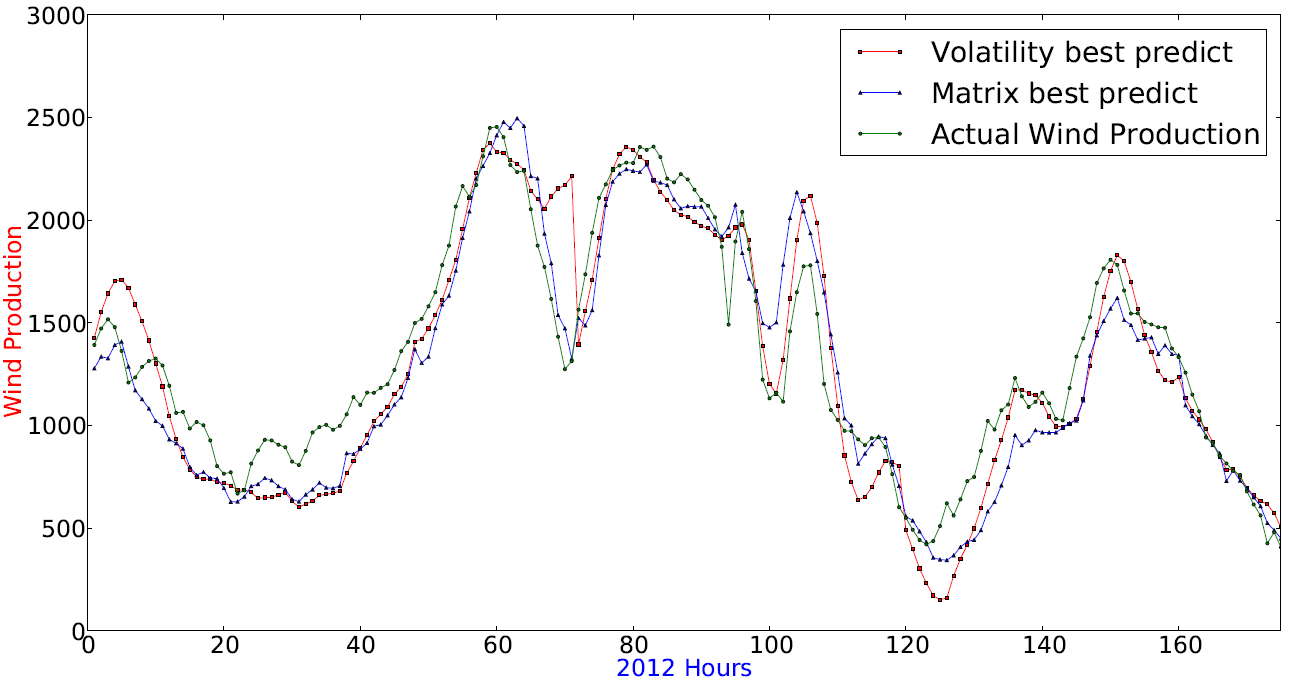
\includegraphics[width=0.99\linewidth]{billeder/bestVolatilityVsMatrixGraph.png}
\caption{Wind production prediction for hours 0-175 in 2012 with historical volatility as input}
\label{fig:bestVolatilityVsMatrixGraph}
\end{figure} 

A noticeable difference from the above graph is how the volatility approach under-shoots its targets in the bottom of many curves compared to the matrix approach in both Figure~\ref{fig:bestVolatilityVsMatrixGraph} and~\ref{fig:bestVolatilityVsMatrixGraph350-525}. It moves more rapidly from top to bottom. Another thing worth mentioning from Figure~\ref{fig:bestVolatilityVsMatrixGraph350-525} is how the addition of historical volatility is capable of predicting all the way to the top in 415 and 480 compared to the standard matrix prediction indicated by the blue line. The under- and overshooting compared to the matrix only prediction is also verified in Figure~\ref{volatilityBest700-1000}.

\begin{figure}[H]
\centering
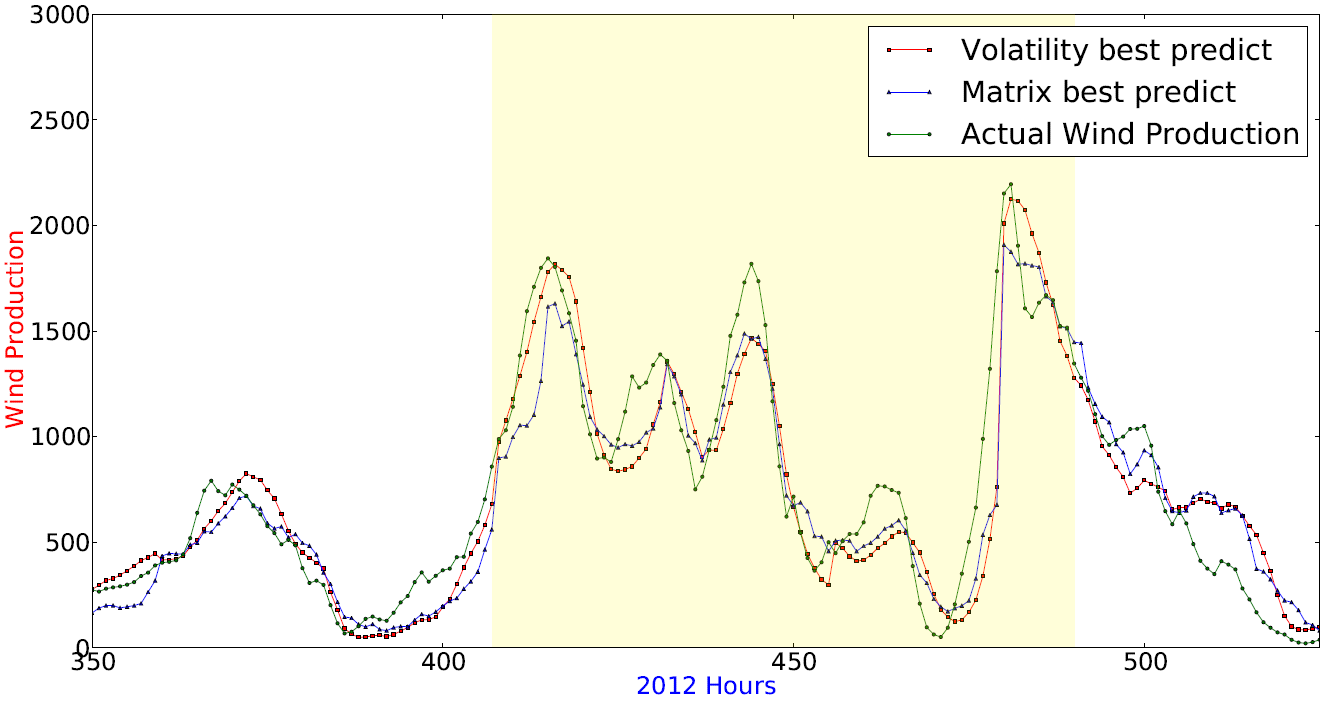
\includegraphics[width=0.99\linewidth]{billeder/bestVolatilityVsMatrixGraph350-525.png}
\caption{Wind production prediction for hours 350-525 hours in 2012 with historical volatility as input}
\label{fig:bestVolatilityVsMatrixGraph350-525}
\end{figure} 

\begin{figure}[H]
\centering
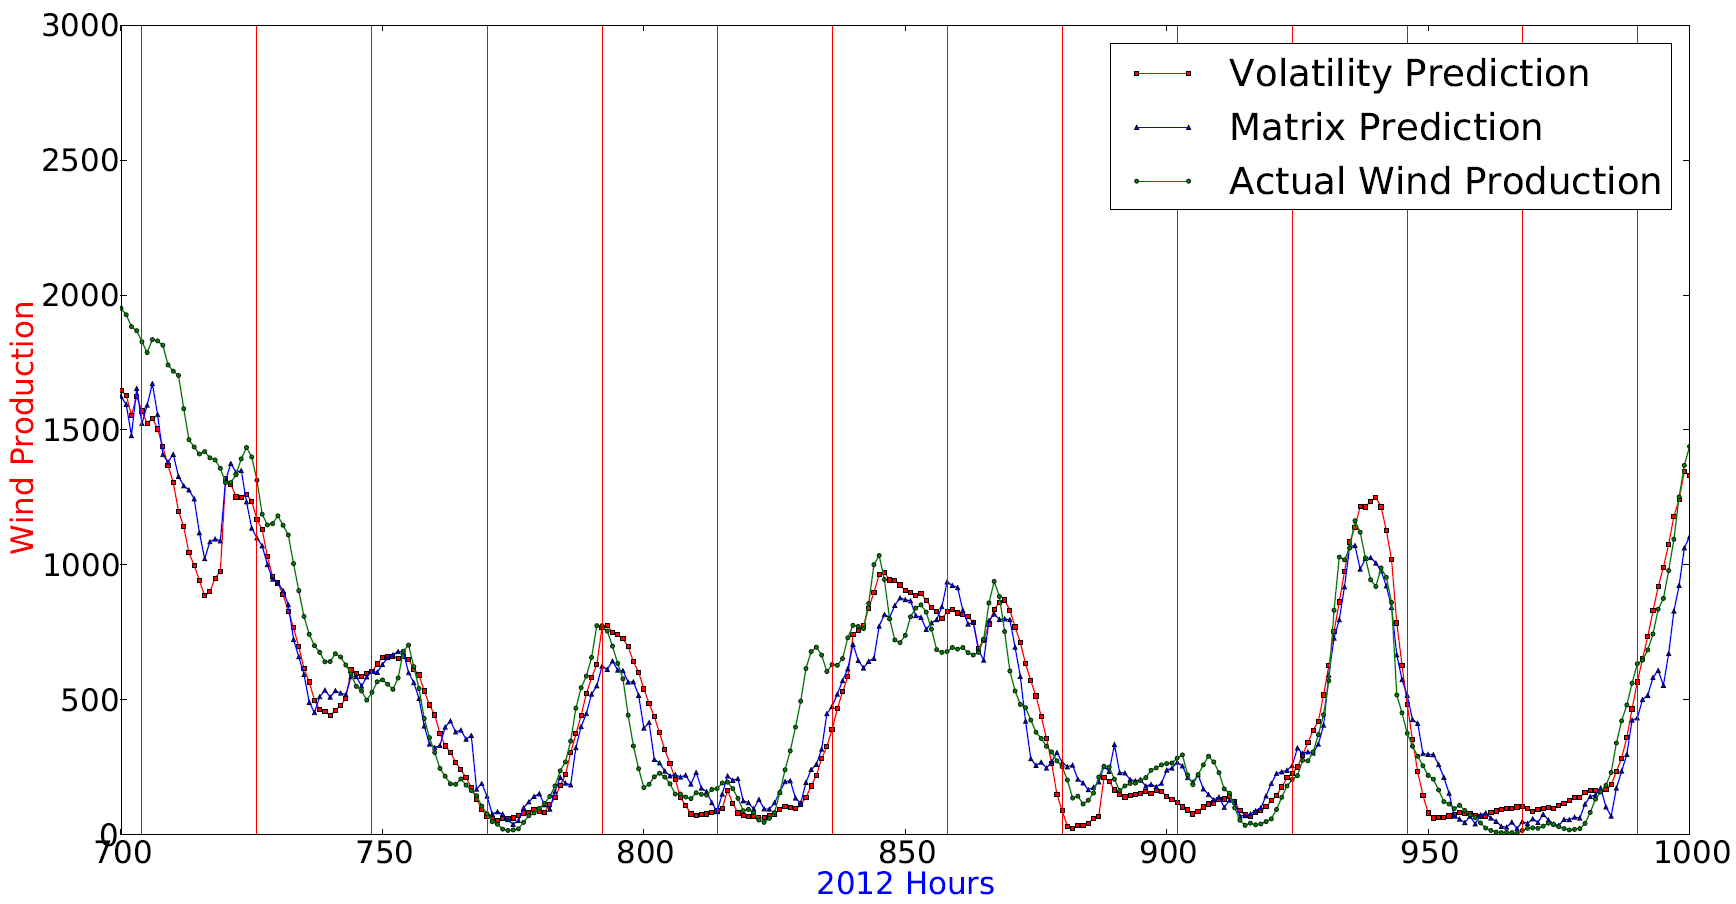
\includegraphics[width=0.99\linewidth]{billeder/volatilityBest700-1000.png}
\caption{Wind production prediction for hours 700-1000 hours in 2012 with historical volatility as input}
\label{fig:volatilityBest700-1000}
\end{figure} 

\subsubsection{Skewness}
Skewness is a calculation of how much a distribution leans to one side of the mean which is described in more detail in Section~\ref{sec:skewness}. What is important to identify is again how many previous hours to include in the calculation of the skew in order to get the best picture of what side the curve is currently leaning towards. Table~\ref{table:skewnessHours} shows results where the best fit is found to be 16 hours. This will be basis for further testing when trying to use the methods in combination to see if any of them can augment each other. At first glance skewness does not seem to improve much but it will need testing when put together with the other calculations.

\begin{center}
\begin{longtable}{|c|c|c|c|}
\hline
\textbf{Hours} & \textbf{MAPE} & \textbf{MAE} & \textbf{\% Correct Direction}\\
\hline
\endfirsthead
\multicolumn{4}{c}%
{\tablename\ \thetable\ -- \textit{Continued from previous page}} \\
\hline
\textbf{Hours} & \textbf{MAPE} & \textbf{MAE} & \textbf{\% Correct Direction}\\
\hline
\endhead
\hline \multicolumn{4}{r}{\textit{Continued on next page}} \\
\endfoot
\endlastfoot
\arrayrulecolor{light-gray}
16 & 18,88\% & 125,85 & 69\% \\ \hline
4 & 19,13\% & 127,52 & 70\% \\ \hline
24 & 19,45\% & 129,63 & 69\% \\ \hline
8 & 19,68\% & 131,18 & 68\% \\ \hline
12 & 19,69\% & 131,26 & 68\% \\ \hline
6 & 19,73\% & 131,51 & 68\% \\ \hline
20 & 20,23\% & 134,81 & 67\% \\ \hline
2 & 20,9\% & 139,33 & 66\% \\ \hline
\caption{Prediction With Skewness and different hours}
\label{table:skewnessHours}
\end{longtable}
\end{center}

Figure~\ref{fig:bestSkewnessGraph} shows the first 175 hours when using skewness as input compared to standard matrix when predicting. The matrix with skewness is much similar to the one without and will not be discussed in further detail. 

\begin{figure}[H]
\centering
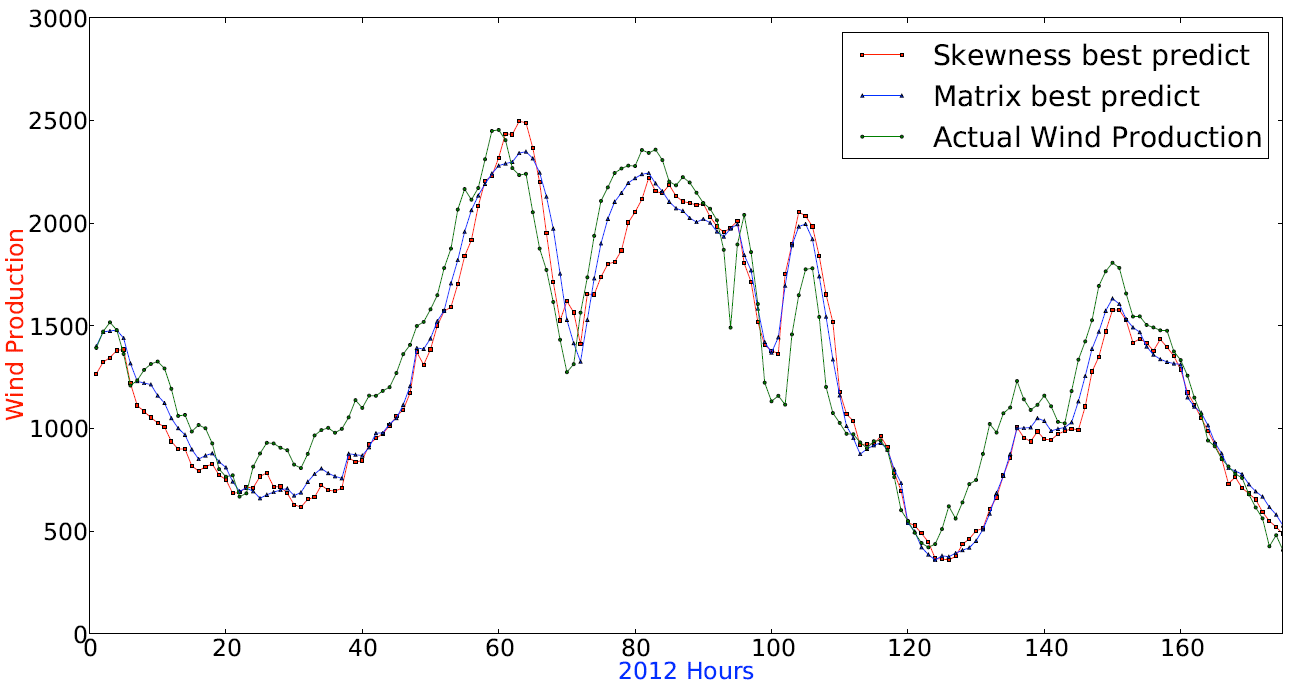
\includegraphics[width=0.99\linewidth]{billeder/bestSkewnessGraph.png}
\caption{Wind production prediction for 175 hours in 2012 with skewness as input}
\label{fig:bestSkewnessGraph}
\end{figure}    

\subsubsection{Slope calculation}
\label{sec:windPowerSlopeCalc}
The experiment covers basic slope calculation of the curve. The intention is to get a notion of how much the previous productions have been going upwards before a particular hour. It captures how the slopes in general relate to the wind power production --- does a very steep slope in general affect the production to go up or not? The calculation has been attempted on different hours to identify the best place to calculate the slope from. Table~\ref{table:curveAnalysisHours} shows that the slope calculation as input does not work as intended. All MAEs show worse results compared to the same predictions without it.

\begin{center}
\begin{longtable}{|c|c|c|c|c|}
\hline
\textbf{Hours} & \textbf{MAPE} & \textbf{MAE} & \textbf{\% Correct Direction} \\
\hline
\endfirsthead
\multicolumn{4}{c}%
{\tablename\ \thetable\ -- \textit{Continued from previous page}} \\
\hline
\textbf{Hours} & \textbf{MAPE} & \textbf{MAE} & \textbf{\% Correct Direction} \\
\hline
\endhead
\hline \multicolumn{4}{r}{\textit{Continued on next page}} \\
\endfoot
\endlastfoot
\arrayrulecolor{light-gray}
20 & 20,0\% & 133,27 & 68\% \\ \hline
16 & 20,03\% & 133,52 & 67\% \\ \hline
12 & 20,56\% & 137,05 & 67\% \\ \hline
8 & 21,01\% & 140,0 & 70\% \\ \hline
24 & 21,98\% & 146,5 & 66\% \\ \hline
6 & 22,28\% & 148,5 & 67\% \\ \hline
2 & 22,75\% & 151,62 & 67\% \\ \hline
4 & 24,17\% & 161,12 & 66\% \\ \hline
\caption{Results for slope calculation as input on different previous hours}
\label{table:curveAnalysisHours}
\end{longtable}
\end{center}

The impact of slope is illustrated in the first 175 of 2012 and can be seen in Figure~\ref{fig:basicCurveAnalysisGrapho}. The best result from Table~\ref{table:curveAnalysisHours} calculates the slope from the previous 20 hours and pink overlay (48-70) illustrates that it has a hard time identifying when to stop moving up since it has been moving up for so long. The 24-ahead prediction starts at 48 just before the drop and since the slope calculation is based on the last 20 hours it does not identify the shift --- it has a steep slope and points the overall generalization upwards since steep slopes in most cases result in ascending curves except when at the very top of one. The opposite happens in the blue overlay (hours 70-80) where it does not know when to stop and undershoots. It stands in contrast to the prediction without curve indicated by the blue line.

\begin{figure}[H]
\centering
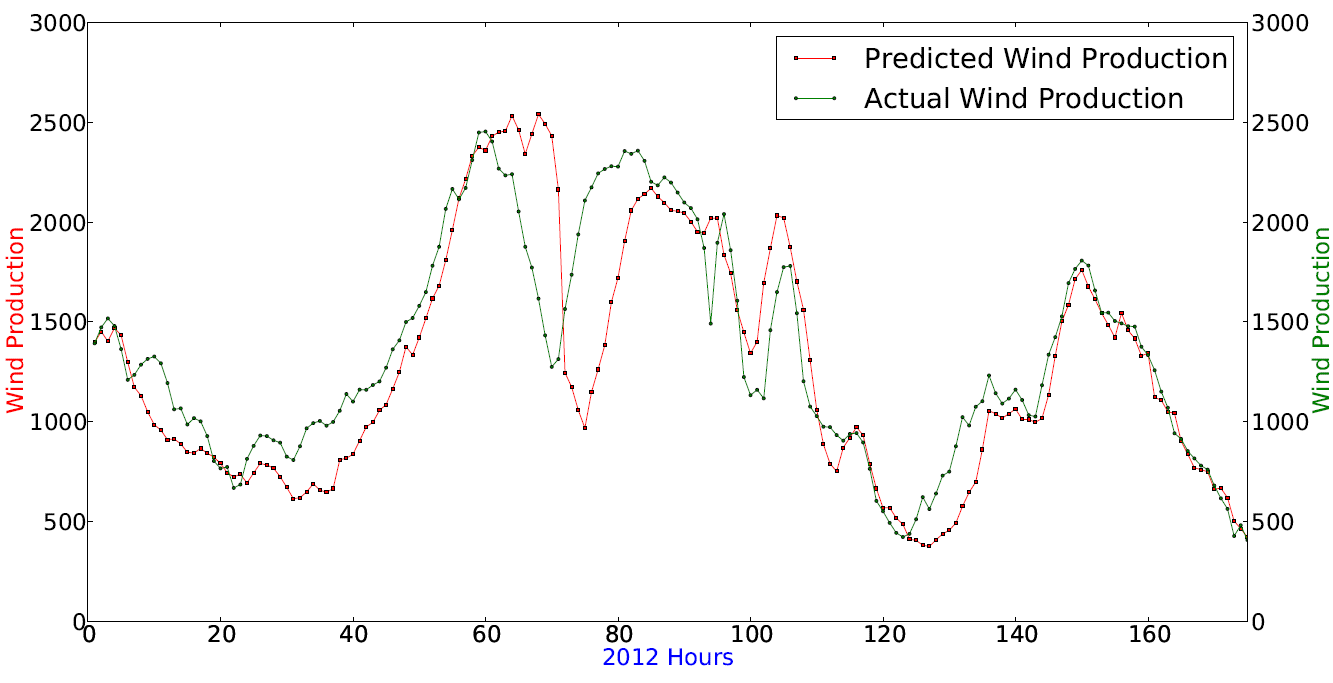
\includegraphics[width=0.99\linewidth]{billeder/curveAnalysisWindProduction.png}
\caption{Wind production prediction for 175 hours in 2012 with slope as input}
\label{fig:basicCurveAnalysisGrapho}
\end{figure} 

It was stated that the 24-ahead prediction was the contributing factor to the elevation of error of the curve approach. To verify this the 1-hour-ahead forecasting with slope has been performed which obtains a MAE of 56,6. The graph can be seen in Figure~\ref{fig:curveOneAheadvs24Ahead} where the curve fitting as expected is significantly better. It can be concluded that the use of slope helps elevate the error which is not a desirable feature. We will attempt to combine it with the other calculated approaches to investigate if any of them augment each others ability.

\begin{figure}[H]
\centering
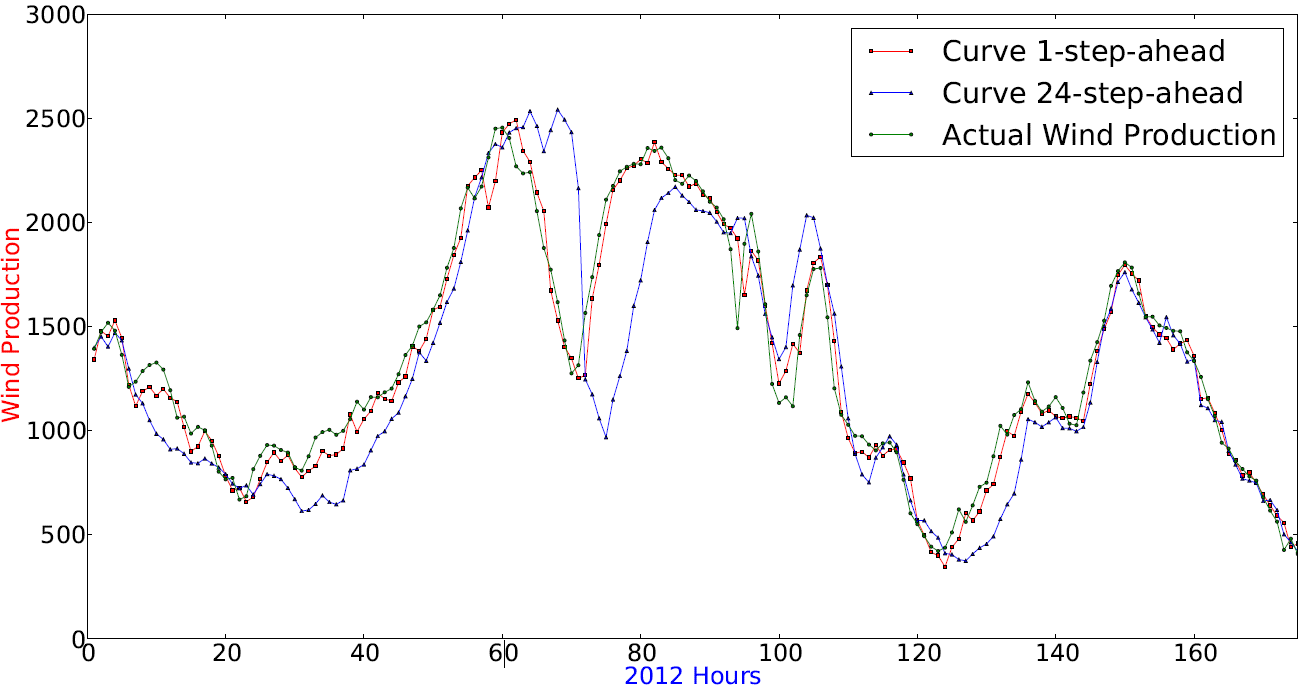
\includegraphics[width=0.99\linewidth]{billeder/curveOneAheadvs24Ahead.png}
\caption{1-step vs. 24-step ahead wind power predictions with curve}
\label{fig:curveOneAheadvs24Ahead}
\end{figure}   

\subsubsection{Combining the approaches}
\label{sec:combiningTheApproachesWP}
Experiments with combinations of the approaches have been performed to investigate whether or not any of them can possibly augment each other. Furthermore, adding historical productions as input has been tried as presented in Section~\ref{sec:scatterPaper} and discussed in Section~\ref{sec:scatterStrategy}. The approach adds 3 inputs for the wind power from one day ago, 3 inputs from the production one week ago, one input from the production two weeks ago, one input from the production three weeks ago and one last input from four weeks ago. The purpose is letting the network itself capture the price development over time instead of calculating it beforehand. Experiment results from each approach is in Table~\ref{table:comparisonStatistics} where the historical volatility with a smoothing factor of 0,70 and 6 previous hours outperforms the other approaches. 

\begin{center}
\begin{longtable}{|c|c|c|c|}
\hline
\textbf{Type} & \textbf{MAPE} & \textbf{MAE} & \textbf{\% CD} \\
\hline
\endfirsthead
\multicolumn{4}{c}%
{\tablename\ \thetable\ -- \textit{Continued from previous page}} \\
\hline
\textbf{Type} & \textbf{MAPE} & \textbf{MAE} & \textbf{\% CD} \\
\hline
\endhead
\hline \multicolumn{4}{r}{\textit{Continued on next page}} \\
\endfoot
\endlastfoot
\arrayrulecolor{light-gray}
Volatility, 0,70 as smoothing on 6 hours & 18,28\% & 121,81 & 73\% \\ \hline
Skewness with 16 hours & 18,88\% & 125,85 & 69\% \\ \hline
Scatter of prices & 20.0\% & 134,7 & 68\% \\ \hline
Slope as input with 20 hours & 20,0\% & 133,27 & 68\% \\ \hline
\caption{Comparison of the approaches}
\label{table:comparisonStatistics}
\end{longtable}
\end{center}

Skewness and curve in combination with each other achieves the best result but does not improve the results from Table~\ref{table:theWindProdInputParamsTop10WithMatrix}. The problem is most likely that the analysis of the curve gets to high priority in the generalization when trying to predict 24-ahead. When trying to predict a scenario totally different from what has just been seen, the calculated inputs will pull the generalization in the direction of the previous which we can see from Figure~\ref{fig:bestStatisticalApproachGraph}. Without the calculated inputs the generalization relies heavily on wind speed which was established in the analysis in Section~\ref{sec:windPowerAnalysis} but this will be contradicted by the calculated inputs that believe the curve to be heading in another direction because we are at the edge. The prediction relies heavily on where to predict from. The best of the calculated approaches based on the above results are volatility as only input with a MAE of 121,81.

\begin{figure}[H]
\centering
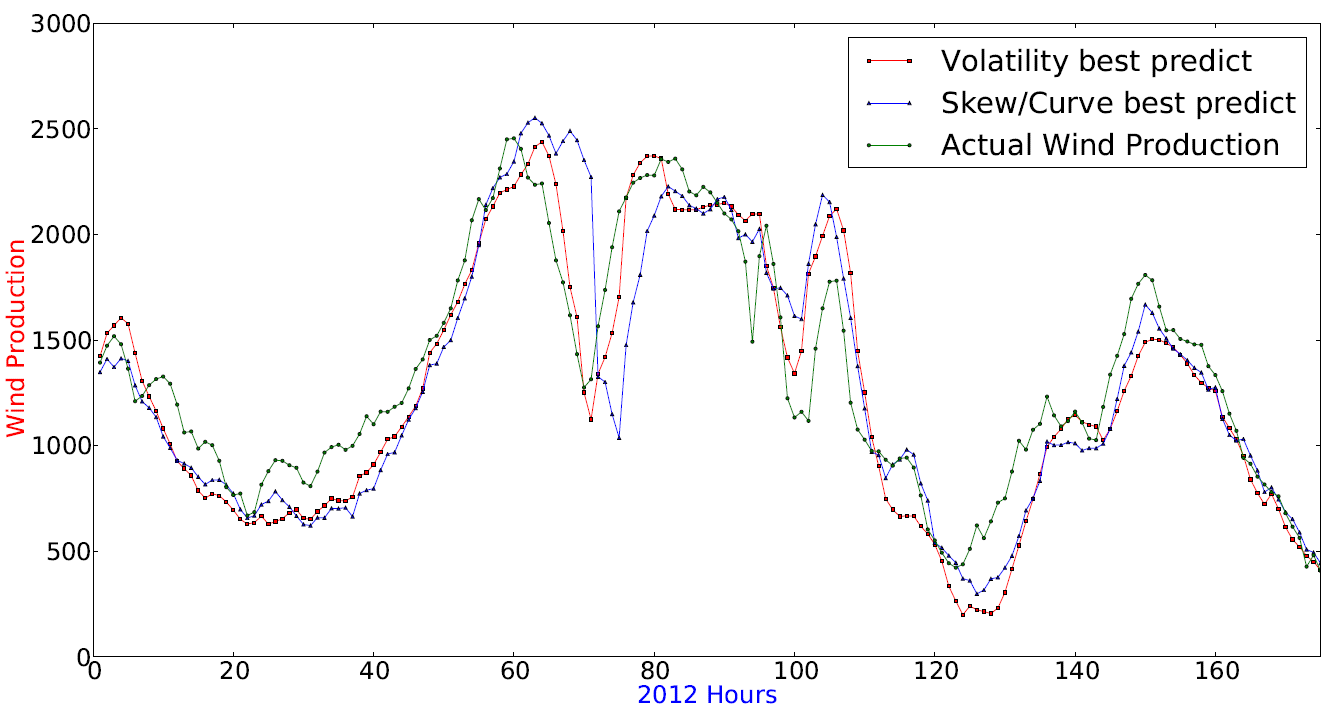
\includegraphics[width=0.99\linewidth]{billeder/bestStatisticalApproachGraph.png}
\caption{Wind production prediction for hours 120-144 in 2012 with historical volatility}
\label{fig:bestStatisticalApproachGraph}
\end{figure} 

\begin{center}
\begin{longtable}{|c|c|c|c|c|c|c|c|}
\hline
\textbf{Vola} & \textbf{Skew} & \textbf{Scat} & \textbf{Curve} & \textbf{MAPE} & \textbf{MAE} & \textbf{\% Rank} & \textbf{\% CD} \\
\hline
\endfirsthead
\multicolumn{8}{c}%
{\tablename\ \thetable\ -- \textit{Continued from previous page}} \\
\hline
\textbf{Vola} & \textbf{Skew} & \textbf{Scat} & \textbf{Curve} & \textbf{MAPE} & \textbf{MAE} & \textbf{\% Rank} & \textbf{\% CD} \\
\hline
\endhead
\hline \multicolumn{8}{r}{\textit{Continued on next page}} \\
\endfoot
\endlastfoot
\arrayrulecolor{light-gray}
 &  \x &  &  \x & 19,76\% & 131,69 & 0,0\% & 69\% \\ \hline
 \x &  \x &  &  & 20,96\% & 139,73 & 6,11\% & 72\% \\ \hline
 \x &  \x &  \x &  & 21,65\% & 144,33 & 9,6\% & 72\% \\ \hline
 \x &  \x &  &  \x & 22,35\% & 148,94 & 13,1\% & 72\% \\ \hline
 \x &  &  \x &  & 22,4\% & 149,31 & 13,38\% & 71\% \\ \hline
 \x &  &  &  \x & 22,93\% & 152,85 & 16,07\% & 71\% \\ \hline
 &  \x &  \x &  & 23,37\% & 155,74 & 18,26\% & 72\% \\ \hline
 &  &  \x &  \x & 23,44\% & 156,25 & 18,65\% & 72\% \\ \hline
 &  \x &  \x &  \x & 23,66\% & 157,69 & 19,74\% & 72\% \\ \hline
 \x &  \x &  \x &  \x & 25,74\% & 171,54 & 30,26\% & 71\% \\ \hline
 \x &  &  \x &  \x & 26,06\% & 173,69 & 31,89\% & 71\% \\ \hline
\caption{All combinations of statistical features on the best from matrix}
\label{table:idealCombinationStatistic}
\end{longtable}
\end{center}

\subsubsection{Using Best Approach on Top-3}
Table~\ref{table:topFromMatrixWithStatistics} shows volatility applied on the top 3 input combinations with matrix from Table~\ref{table:theWindProdInputParamsTop10WithMatrix}. It is first of all noticeable that the top 3 positions are the same as in all of the combination tests. Secondly, the results are in general improved. The best ranked from ~\ref{table:idealCombinationStatistic} is the same as the best ranked here. The results emphasize the best input combinations and the improvement by adding volatility as input.     

\begin{center}
\begin{longtable}{|c|c|c|c|c|c|c|c|c|c|c|c|}
\hline
\textbf{WS} & \textbf{AD} & \textbf{C} & \textbf{T} & \textbf{WD} & \textbf{L-P} & \textbf{ToD} & \textbf{MAE} & \textbf{\% Rank} &  \textbf{H1} & \textbf{H2} & \textbf{\% CD} \\
\hline
\endfirsthead
\multicolumn{12}{c}%
{\tablename\ \thetable\ -- \textit{Continued from previous page}} \\
\hline
\textbf{WS} & \textbf{AD} & \textbf{C} & \textbf{T} & \textbf{WD} & \textbf{L-P} & \textbf{ToD} & \textbf{MAE} & \textbf{\% Rank} &  \textbf{H1} & \textbf{H2} & \textbf{\% CD} \\
\hline
\endhead
\hline \multicolumn{12}{r}{\textit{Continued on next page}} \\
\endfoot
\endlastfoot
\arrayrulecolor{light-gray}
 \x &  &  &  \x &  &  \x &  \x (m) & 121,81 & 0,0\% & 16 & 13 & 73\& \\ \hline
 \x &  \x &  &  &  &  \x &  \x (m) & 125,15 & 2,74\% & 9 & 13 & 70\%  \\ \hline
 \x &  \x &  &  &  \x &  \x & \x (m) & 128,67 & 5,63\% & 12 & 15  & 72\%\\ \hline
\caption{Volatility applied in top 3 from matrix}
\label{table:topFromMatrixWithStatistics}
\end{longtable}
\end{center}

\subsubsection{Best prediction graph}
Section~\ref{sec:predictionHistVol} covers a more thorough analysis and the best prediction graphs can be seen in Figures~\ref{fig:bestVolatilityVsMatrixGraph} and~\ref{fig:bestVolatilityVsMatrixGraph350-525}. The slope prediction clarified the problem with predicting 24-step-ahead and the elevated error. It was more obvious for curve than for the other predictions but it is applicable for all predictions since every predicted hour uses the previous prediction as input. It is not the same as the 24th hour is always the worst because the prediction can correct itself during the 24 hours which is also seen in Figure~\ref{fig:bestVolatility120to144} even though the volatility predicting under-shoots in the beginning. The figure shows that the addition of volatility moves faster from top to bottom and is more accurate in high numbers than low.
This is also seen in Figure~\ref{fig:bestVolatility408to432}. Since MAE is the error measure better accuracy in the high numbers will contribute to a better average MAE even though the low numbers are worsened. It is a trade-off between the desire to predict low or high wind power productions but here we strive to lower the overall MAE of the predictions. The trade-off is much controlled of use scenarios which will not be covered here.

\begin{figure}[H]
\centering
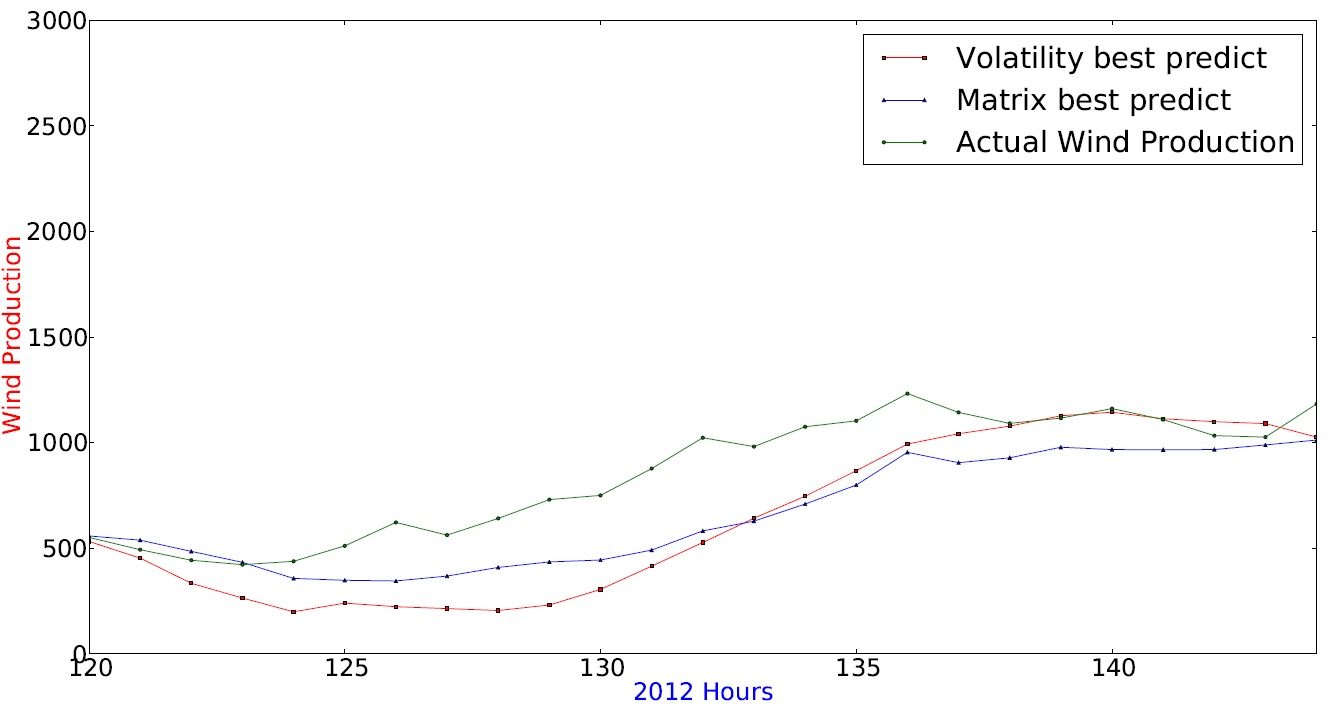
\includegraphics[width=0.99\linewidth]{billeder/bestVolatility120to144.png}
\caption{Wind production prediction for hours 120-144 in 2012 with historical volatility}
\label{fig:bestVolatility120to144}
\end{figure} 

\begin{figure}[H]
\centering
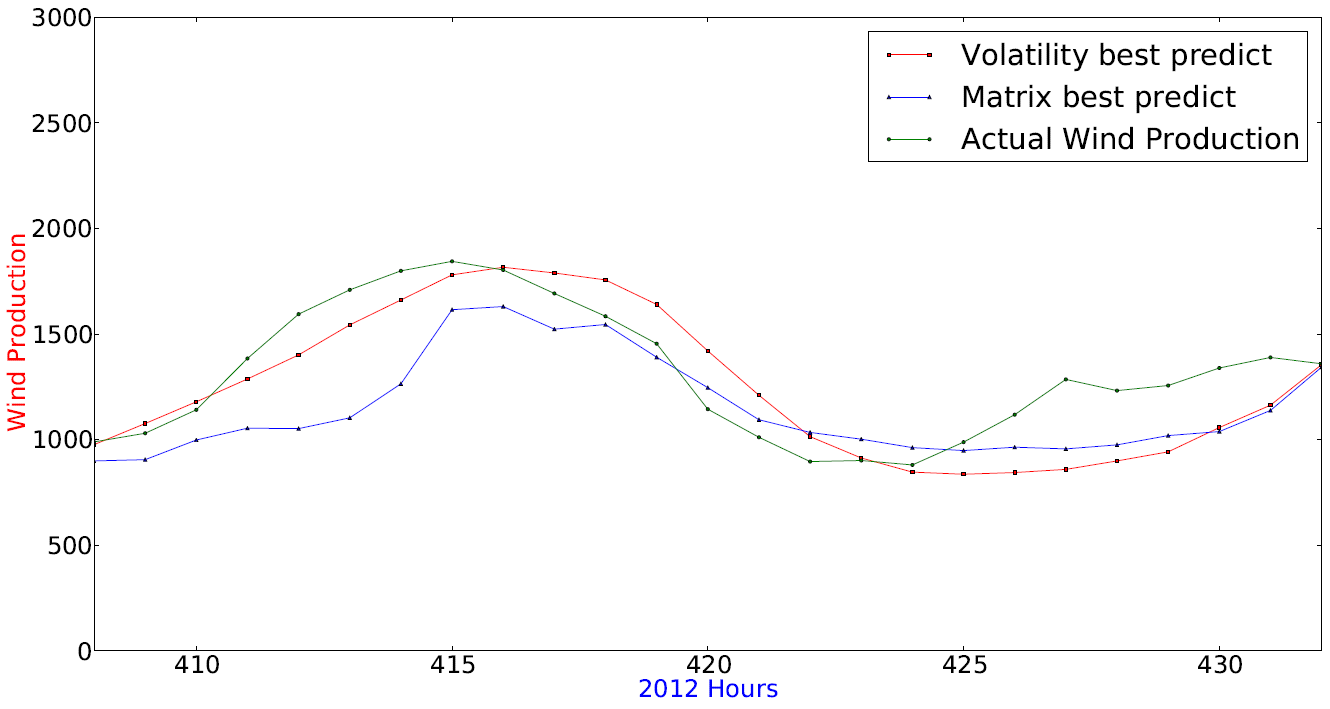
\includegraphics[width=0.99\linewidth]{billeder/bestVolatility408to432.png}
\caption{Wind production prediction for hours 408-432 in 2012 with historical volatility}
\label{fig:bestVolatility408to432}
\end{figure} 

\subsubsection{Conclusion}
Various calculated inputs have been used as input in an attempt to augment the existing generalization based on the meteorological factors. 

\begin{enumerate}
\item Historical volatility by itself showed to be the best calculated input approach with a smoothing factor of 0,70 based on 6 previous hours. The prediction curve moved more rapidly than without any calculated inputs and showed to be better in the higher numbers than low which is what contributes to the overall decrease in MAE. Trade-offs must be made in relation to the specific task but in this thesis the decrease in MAE when using historical volatility will be considered an improvement. The overall improvement in relation to the corresponding combination without it from Table~\ref{table:theWindProdInputParamsTop10WithMatrix} was 3,52\%.
\item The use of scatter and curve resulted in a worsening in MAE. Curve as input was analysed in some detail and the most obvious problem was related to the 24-step-ahead forecasting. When left before a situation very different from what has been seen lately in the training set the curve approach showed difficulties, e.g. trying to predict from the edge of a very steep slope resulted in the curve input pulling the generalization up because a steep slope in general in the training set results in a rising curve. Skewness showed similar results to prediction without any calculated inputs and was therefore not further analysed.
\item It was expected that the statistical approaches in combination could augment each other because they specialize in different areas. This was proven wrong and the results got significantly worse than the best without any calculated inputs. The calculated features are given to high priority when combined and since it cannot be controlled where to predict from it can cause problems when for instance left to predict from the edge of a curve. 
\end{enumerate}

\newpage

\subsection{Experiment Four - Black Box Optimization}
The purpose of experiment four is to find the best number of epochs and dataset size for training. Black box optimization is a way of fine-tuning the network to obtain the best possible prediction.

\subsubsection{Hypothesis}
The size of the training set and number of epochs influence the prediction and from that assume the following:
\begin{enumerate}
\item It is the assumption that too many epochs will result in an over-fitting over the network and therefore a worse prediction. Too few epochs will be under-fit and also a bad prediction.
\item It is expected that a too big or small dataset will result in worse predictions. Too little data will be hard to generalize upon and too much data can bring too much noise.
\end{enumerate}

\subsubsection{Variables}
The best combination of variables has been concluded from previous experiments and will be the basis for the black box optimization. 

\begin{itemize}
\item Wind speed (WS).
\item Time of day as matrix (ToD).
\item Temperature (T).
\item Last known production (L-P).
\item Historical volatility with 0,70 on 6 previous hours (V).
\end{itemize}

The parameters are tested with the following configurations:

\begin{itemize}
\item Selected values between 1 to 2800 epochs.
\item Training set sizes of 1, 3, 6, 9 and 12 months.
\end{itemize}

\subsubsection{Prediction - Epochs}
The number of epochs influence the prediction significantly which is established in Table~\ref{table:bestPredictionEpochExperiment}. It is obvious that too few epochs will result in the network being "under-trained". It can be seen from 1 and 10 epochs that the initial random weights of the network has not yet been adjusted to reflect the training set and therefore predicts randomly. Furthermore, when the number of epochs reach above 2000 it achieves a worse MAE in general. The best result is obtained by 2-300 epochs but with 1200 right after. The results reflect how different epochs affect the production but also how the network can be under-trained or over-trained by either too many or too few epochs. It is obvious from the table that the time in seconds moves up with the number of epochs. Furthermore, the correct direction percentage has been stable in all of the experiments around 70\% but here it can be seen that training to few epochs will result in the percentage dropping significantly together with the worsening in MAE.


\begin{center}
\begin{longtable}{|c|c|c|c|c|c|}
\hline
\textbf{Epochs} & \textbf{MAPE} & \textbf{MAE} & \textbf{\% Rank} & \textbf{Time (s)} & \textbf{\% Correct Direction} \\
\hline
\endfirsthead
\multicolumn{6}{c}%
{\tablename\ \thetable\ -- \textit{Continued from previous page}} \\
\hline
\textbf{Epochs} & \textbf{MAPE} & \textbf{MAE} & \textbf{\% Rank} & \textbf{Time (s)} & \textbf{\% Correct Direction} \\
\hline
\endhead
\hline \multicolumn{6}{r}{\textit{Continued on next page}} \\
\endfoot
\endlastfoot
\arrayrulecolor{light-gray}
300 & 18,16\% & 121,02 & 0,0\% & 813 & 73,0\% \\ \hline
200 & 18,28\% & 121,81 & 0,65\% & 631 & 73,0\% \\ \hline
1200 & 18,37\% & 122,43 & 1,17\% & 1650 & 71,0\% \\ \hline
1400 & 18,85\% & 125,63 & 3,81\% & 1720 & 72,0\% \\ \hline
400 & 18,9\% & 125,96 & 4,08\% & 1208 & 70,0\% \\ \hline
1100 & 18,95\% & 126,31 & 4,37\% & 1739 & 71,0\% \\ \hline
600 & 19,09\% & 127,23 & 5,13\% & 1483 & 70,0\% \\ \hline
50 & 19,34\% & 128,89 & 6,5\% & 580 & 70,0\% \\ \hline
1500 & 20,2\% & 134,61 & 11,23\% & 2381 & 69,0\% \\ \hline
1300 & 20,68\% & 137,84 & 13,9\% & 1981 & 68,0\% \\ \hline
700 & 20,92\% & 139,45 & 15,23\% & 1152 & 73,0\% \\ \hline
1600 & 21,0\% & 139,95 & 15,64\% & 1720 & 72,0\% \\ \hline
800 & 21,05\% & 140,32 & 15,95\% & 966 & 72,0\% \\ \hline
500 & 21,08\% & 140,49 & 16,09\% & 913 & 72,0\% \\ \hline
150 & 21,18\% & 141,15 & 16,63\% & 669 & 72,0\% \\ \hline
900 & 21,36\% & 142,34 & 17,62\% & 972 & 72,0\% \\ \hline
2200 & 21,47\% & 143,1 & 18,24\% & 1812 & 72,0\% \\ \hline
2600 & 21,52\% & 143,46 & 18,54\% & 3159 & 72,0\% \\ \hline
1800 & 21,58\% & 143,82 & 18,84\% & 2085 & 72,0\% \\ \hline
2400 & 21,59\% & 143,88 & 18,89\% & 2105 & 72,0\% \\ \hline
1000 & 21,78\% & 145,14 & 19,93\% & 1101 & 71,0\% \\ \hline
40 & 22,24\% & 148,21 & 22,47\% & 437 & 71,0\% \\ \hline
2800 & 22,98\% & 153,19 & 26,58\% & 3159 & 72,0\% \\ \hline
2000 & 23,2\% & 154,6 & 27,75\% & 2045 & 71,0\% \\ \hline
20 & 24,0\% & 159,98 & 32,19\% & 441 & 66,0\% \\ \hline
10 & 96,73\% & 644,72 & 432,74\% & 423 & 45,0\% \\ \hline
1 & 149,64\% & 997,34 & 724,11\% & 464 & 50,0\% \\ \hline
\caption{Best prediction with different epochs on same network (H1: 3 and H2: 17)}
\label{table:bestPredictionEpochExperiment}
\end{longtable}
\end{center}

\subsubsection{Prediction - Dataset size}
The size of the dataset has already been discussed during the initial experiments with the best combination of input parameters. Too large training sets can result in over-training as described in\cite{1}, e.g. the dataset contains a lot of different cases and because of that has difficulties when predicting the unseen data of only 24 hours. The over-training consists in the network generalizing upon all cases which can become noise when trying to predict only one of these cases. This corresponds well with wind power production and its high volatility and seasonal. This must be differentiated with over-fitting with too many epochs where weights are being adjusted to the same training set over and over again whereas it in the case of data size simply "knows to much" because too much data makes it hard to generalize. Over-fitting is described in Section~\ref{sec:annSection}. If a training set contains many of the same cases the over-training will be much similar to the one with epochs since it will see the same case over and over again. The weights will be adjusted to that same case again and again and a lower number of epochs are needed. The training set must not be too small because it needs enough cases to generalize upon. Different training set sizes have been tried and the results can be seen in Table~\ref{table:bestPredictionDatasetSizeTest}. The result is as expected since both the small and big datasets are outperformed by the 3 month --- the best have been run again and the new result is much equal to what we saw before. Furthermore, time increases with the size of the data and the 2nd lowest is the best prediction.

\begin{center}
\begin{longtable}{|c|c|c|c|c|c|}
\hline
\textbf{Size} & \textbf{MAPE} & \textbf{MAE} & \textbf{\% Deviation} & \textbf{Time (s)} & \textbf{\% Correctio Direction} \\
\hline
\endfirsthead
\multicolumn{6}{c}%
{\tablename\ \thetable\ -- \textit{Continued from previous page}} \\
\hline
\textbf{Size} & \textbf{MAPE} & \textbf{MAE} & \textbf{\% Deviation} & \textbf{Time (s)} & \textbf{\% Correctio Direction} \\
\hline
\endhead
\hline \multicolumn{6}{r}{\textit{Continued on next page}} \\
\endfoot
\endlastfoot
\arrayrulecolor{light-gray}
 2200 & 18,4\% & 122,65 & 0,0\% & 631 & 72\% \\ \hline
 8600 & 22,03\% & 146,83 & 19,7\% & 1585 & 72\% \\ \hline
 4200 & 23,56\% & 157,01 & 28,01\% & 855 & 71\% \\ \hline
 1000 & 24,72\% & 164,73 & 34,31\% & 462 & 70\% \\ \hline
 6600 & 26,46\% & 182,31 & 48,64\% & 908 & 70\% \\ \hline
\caption{Best prediction with different training set sizes}
\label{table:bestPredictionDatasetSizeTest}
\end{longtable}
\end{center}

\subsubsection{Hidden Layers and Neurons}
Done by pruning. Is it necessary to say something about the network size or can we rely on the literature telling us that pruning is a tool to find the best network?

\subsubsection{Prediction Graphs}
\label{sec:windPowerBestPredictionGraphs}
The best prediction obtains a MAE of 121 with 300 epochs. Due to the random initialization of weights in the Artificial Neural Network the prediction will vary from time to time. Table~\ref{table:bestPredictionDatasetSizeTest} show how the best prediction changed to 122,65 but still fairly close to 121,02 --- this must be taken into consideration and the subject will be addressed in the discussion of results. The experimental results are not 100\% definitive but they have shown clear tendencies in what works and what does not. 

A whole year (as used here) contains the different seasonal impacts but at the same time many similar days so that the same situations are predicted more than once --- the point is of course to cover as different cases as possible but at the same time to reduce randomness by predicting the same (here, similar) more than once. The figures~\ref{fig:bestWPPredictWinter}, ~\ref{fig:bestWPPredictSpring}, ~\ref{fig:bestPredictWPSummer} and ~\ref{fig:bestPredictWPFall} show examples of the behaviour in different seasons and how the prediction is able to handle them. One thing that is noticeable is during fall in the falling curve from 7150-7250 --- it shows what have been stated before, namely that the prediction has trouble when undertaking high volatility (as mentioned in Section~\ref{sec:bestInputCombiGraph} significant volatility makes it harder to predict). The graphs also show the need for predicting a whole year due to the obvious differences in the wind power behaviour but at the same time illustrate the predictions ability to follow the development of the ideal wind power in different seasons. The results comply well with the purpose of being able to approach the wind power and its trends whilst at the same time identifying wind power influential factors in the Danish electricity market. Furthermore, an improvement in accuracy has been seen throughout the experiments.

\begin{figure}[H]
\centering
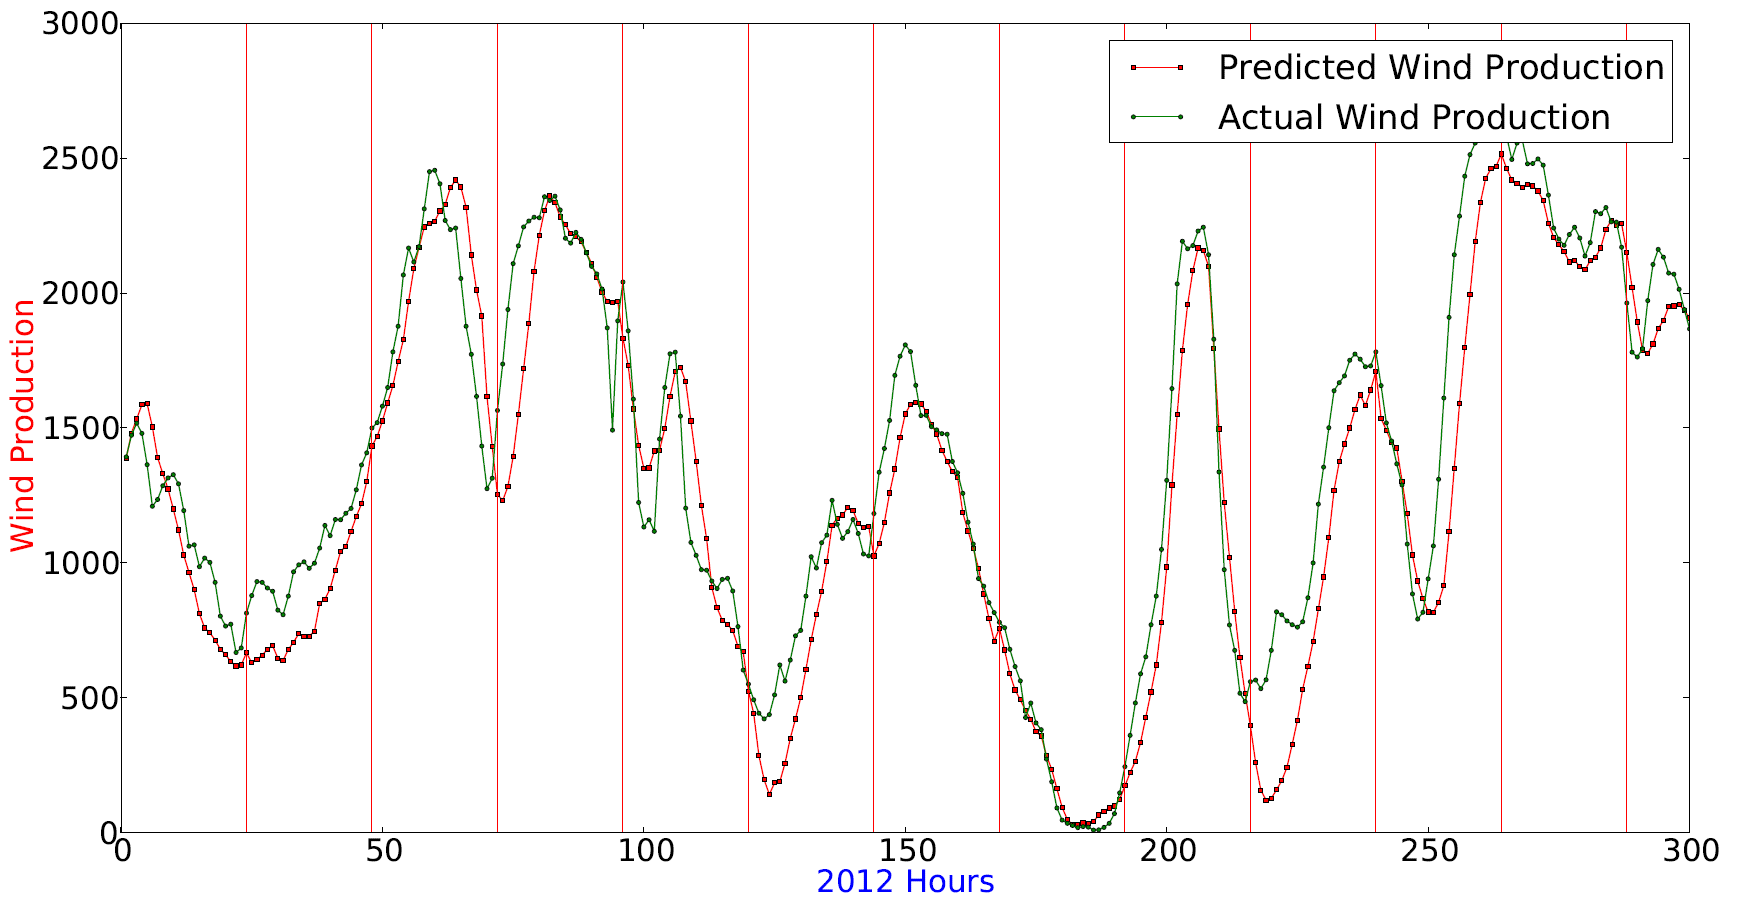
\includegraphics[width=0.99\linewidth]{billeder/bestPossiblePredictionWindProduction0-300.png}
\caption{Best prediction for 300 hours of January (Winter)}
\label{fig:bestWPPredictWinter}
\end{figure}

\begin{figure}[H]
\centering
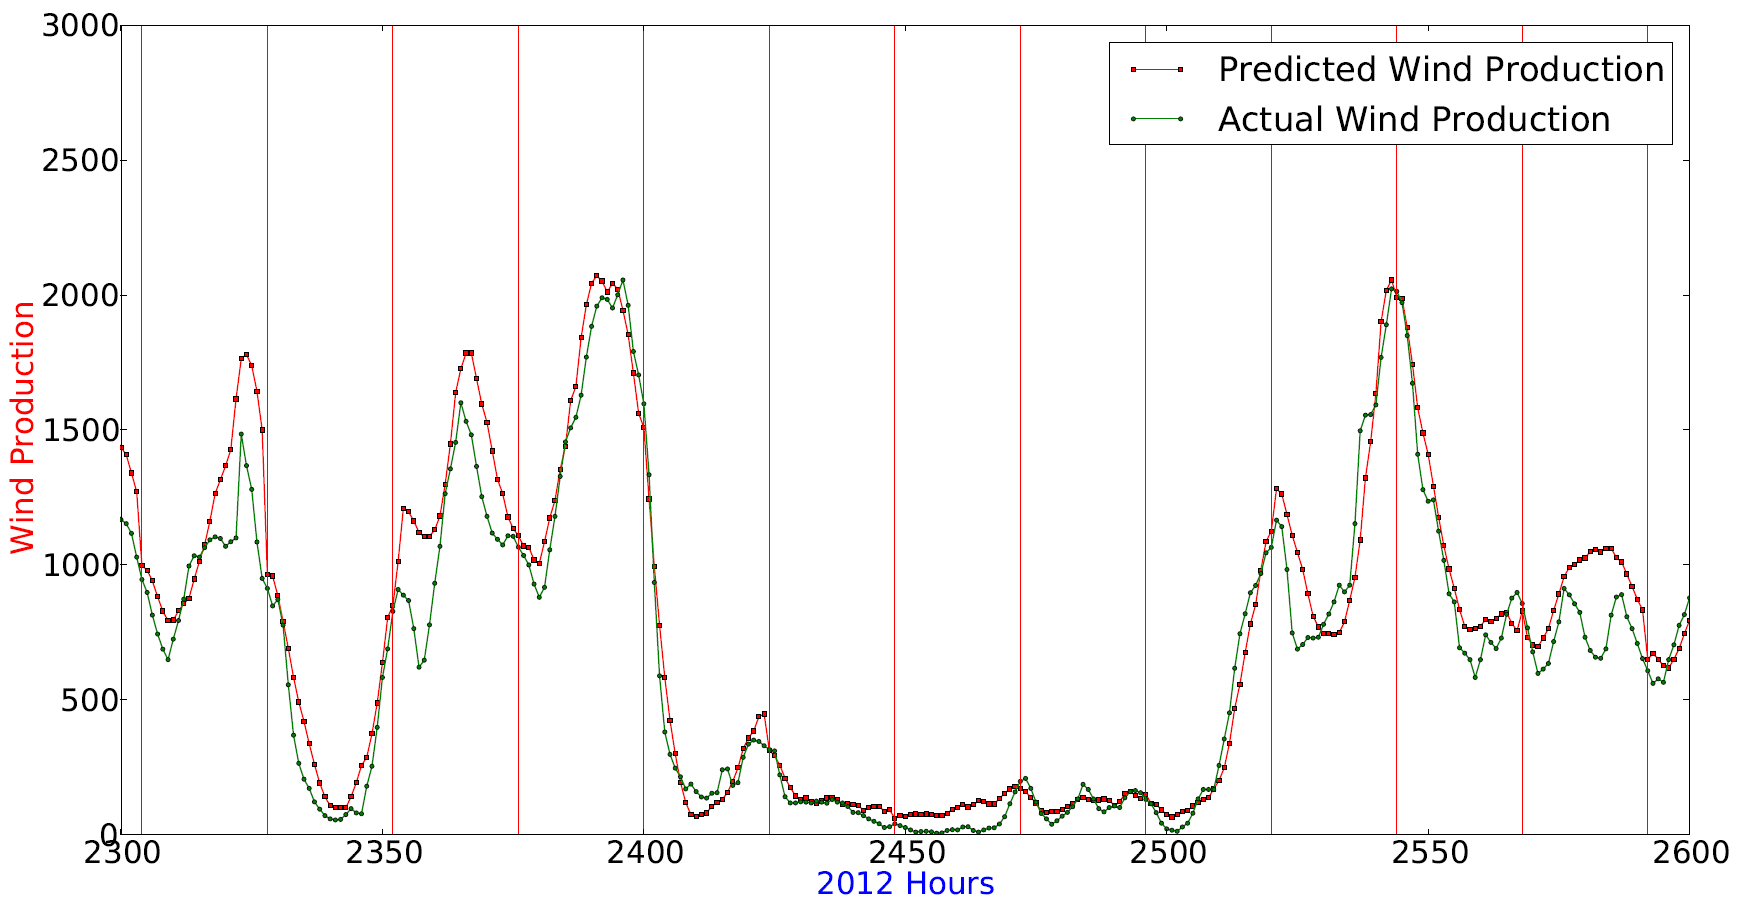
\includegraphics[width=0.99\linewidth]{billeder/bestPossiblePredictionWindProduction2300-2600_April_Spring.png}
\caption{Best prediction for 300 hours of April (Spring)}
\label{fig:bestWPPredictSpring}
\end{figure}

\begin{figure}[H]
\centering
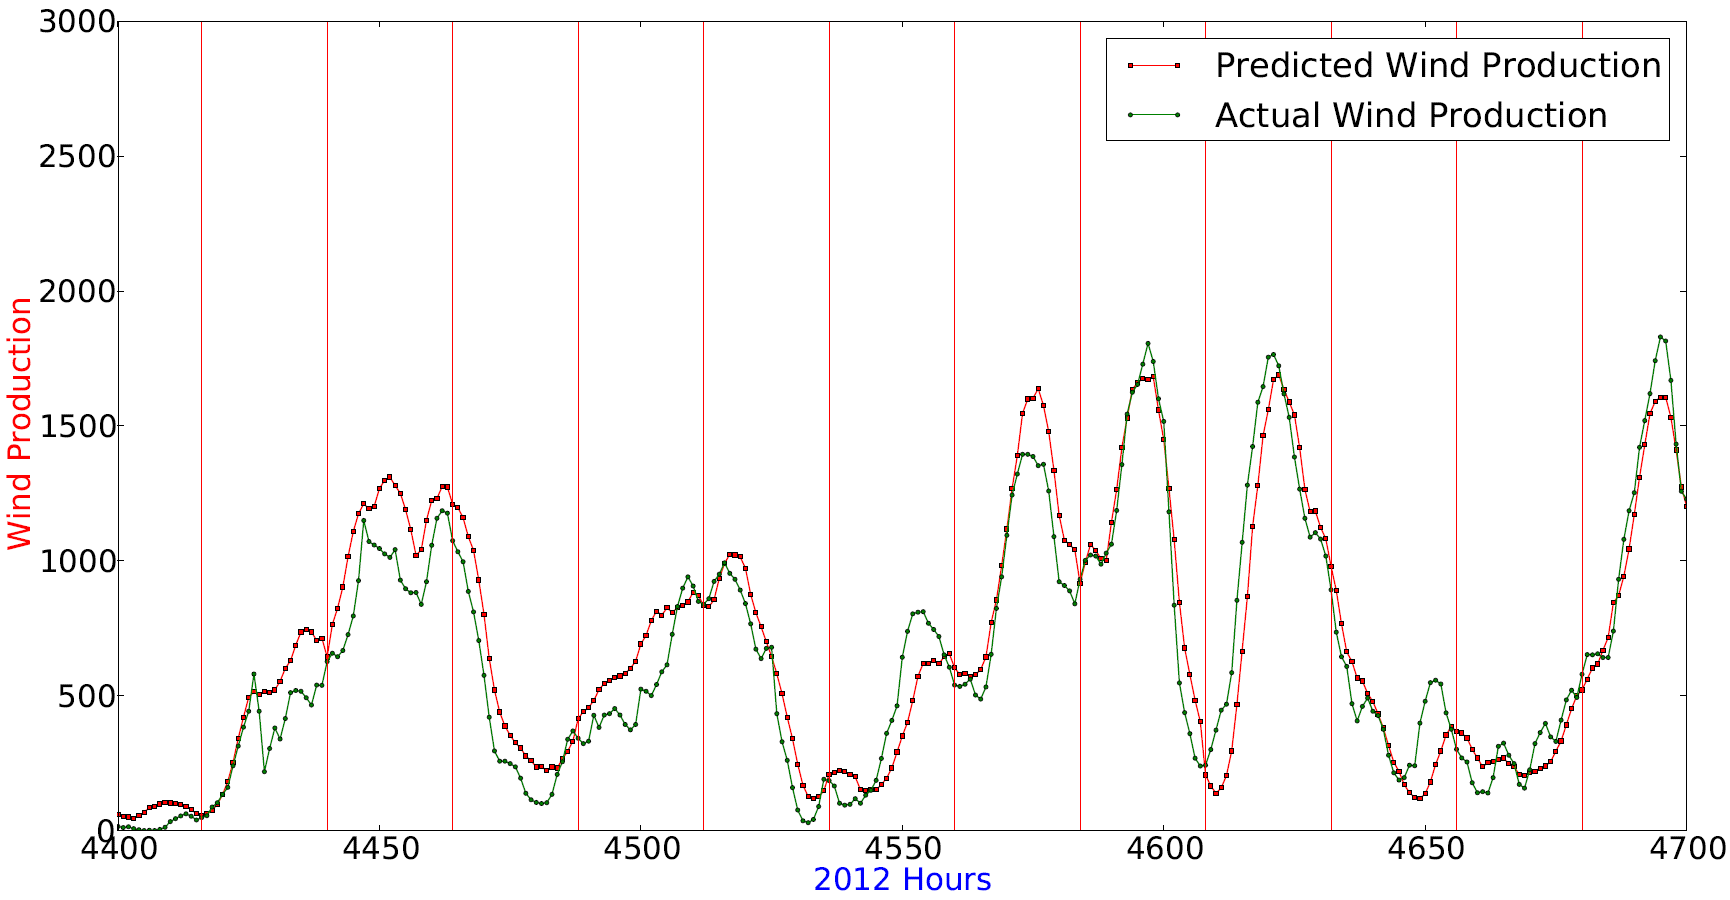
\includegraphics[width=0.99\linewidth]{billeder/bestPossiblePredictionWindProduction4400-4700-Summer.png}
\caption{Best prediction for 300 hours of July (Summer)}
\label{fig:bestPredictWPSummer}
\end{figure}

\begin{figure}[H]
\centering
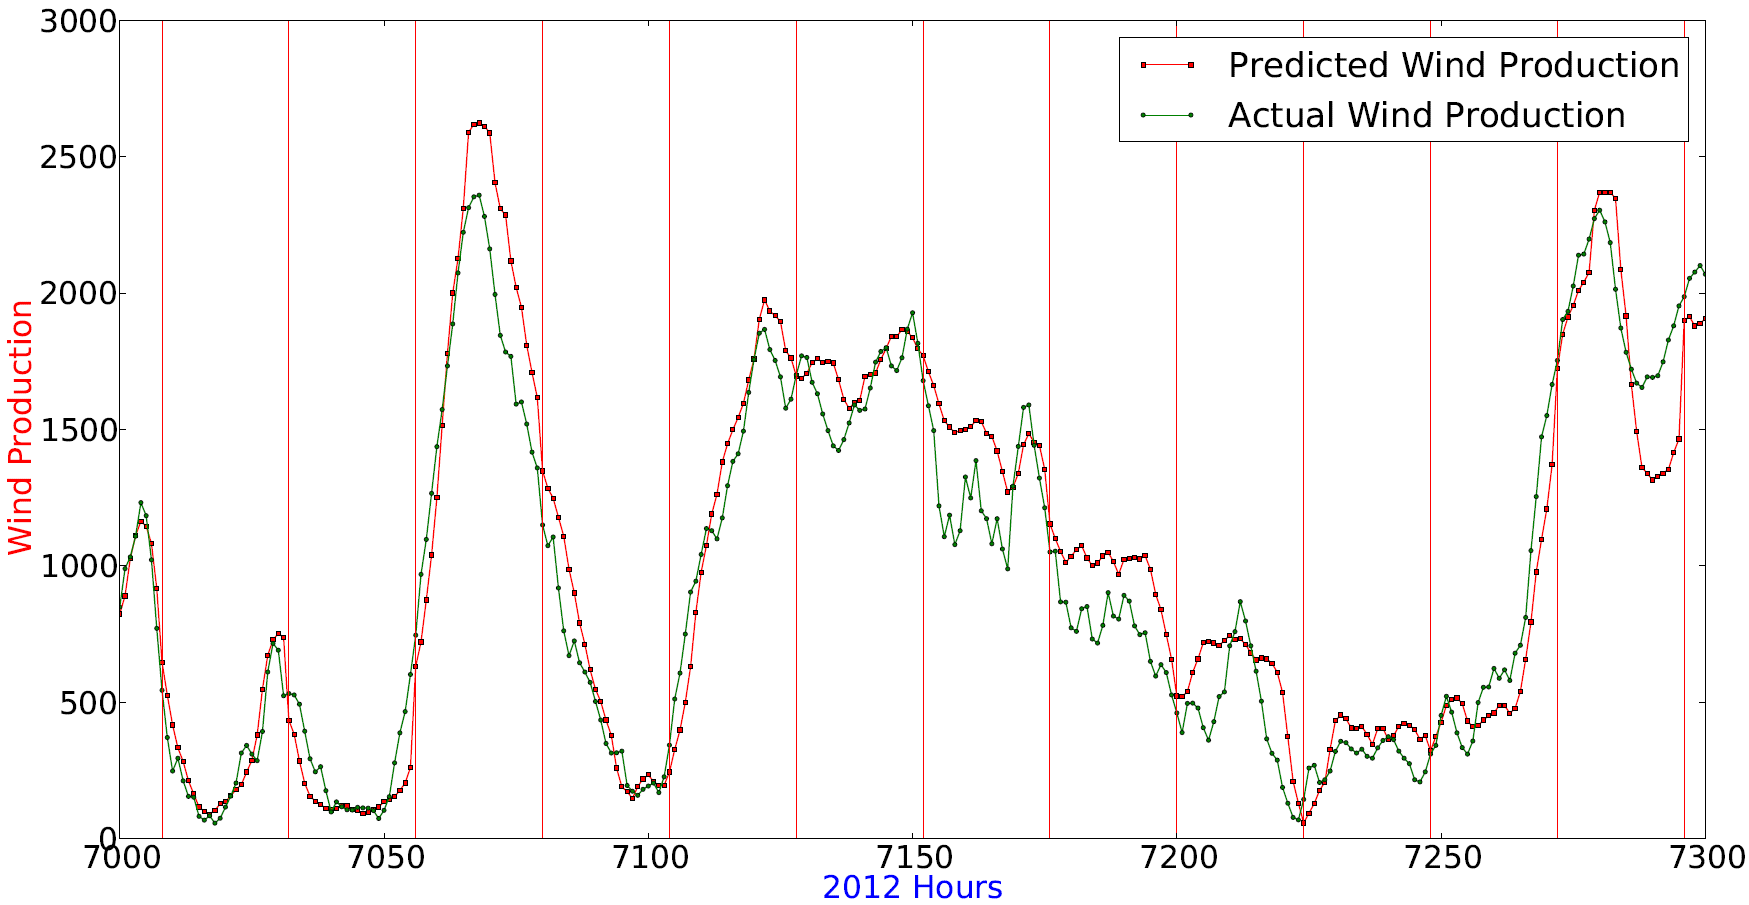
\includegraphics[width=0.99\linewidth]{billeder/bestPossiblePredictionWindProduction7000-7300_Fall.png}
\caption{Best prediction for 300 hours for Oct-Nov (Fall)}
\label{fig:bestPredictWPFall}
\end{figure}

\subsubsection{Conclusion}
Different training set sizes and epochs have been tested and used for prediction.

\begin{enumerate}
\item The results clearly showed the effects of different number of epochs. The expectation was to see under-training and over-training with too many and too few epochs which was confirmed. The best number was 2-300 epochs and the worst 2800, 2000, 20, 10 and 1.
\item Different size of the training set was expected to influence the prediction heavily which was also based on earlier experiences in the first experiments. This was confirmed by the results which showed the best to be on 3 month and the worst to be 3/4 of a year.
\item The predictions graphs presented for the best prediction clearly showed the ability of following the behaviour of the ideal wind power and an improvement in mae in relation to the first experiment. 
\end{enumerate}

\newpage

\subsection{Experiment Five - Step-ahead forecasting}
\label{sec:windPowerExperimentFive}
The purpose is to identify the error in different step-ahead forecasts from 1 hour to 24 hour. In step-ahead forecasting every step is dependent on the prediction from the step just before it but for wind power production that does not necessarily mean that many steps will be the worst since it follows wind speed significantly which will make it possible to correct during the prediction.

\subsubsection{Hypothesis}
It is expected to see an improved error when very few steps is included in the step-ahead forecasting. When the number of steps reach a certain point the results is expected to become more random.

\subsubsection{Step-ahead forecasting}
Table~\ref{table:stepAheadForecastingWindProduction} shows the results from the step-ahead forecasting. It is clear that low numbers until 9 is significantly better than the rest. The expectation was to see a more random distribution when reaching a certain point but there is a tendency in the high numbers in the button and low numbers in the top. The obvious problem with the results is that they are all predicting the same year but as they progress they predict from different starting points which heavily affects the predictions as discussed in Section~\ref{sec:combiningTheApproachesWP}. It makes the results somewhat incomparable since but it still shows that few steps will always be closer to the target until a certain point.

\begin{center}
\begin{longtable}{|c|c|c|c|c|}
\hline
\textbf{Steps ahead} & \textbf{MAPE} & \textbf{MAE} & \textbf{\% Deviation} & \textbf{\% Correct Direction}  \\
\hline
\endfirsthead
\multicolumn{5}{c}%
{\tablename\ \thetable\ -- \textit{Continued from previous page}} \\
\hline
\textbf{Steps ahead} & \textbf{MAPE} & \textbf{MAE} & \textbf{\% Deviation} & \textbf{\% Correct Direction}  \\
\hline
\endhead
\hline \multicolumn{5}{r}{\textit{Continued on next page}} \\
\endfoot
\endlastfoot
\arrayrulecolor{light-gray}
1 & 7,7\% & 51,5 & 0,0\% & 74\%  \\ \hline
2 & 9,85\% & 65,91 & 27,98\% & 70\%  \\ \hline
3 & 11,8\% & 78,94 & 53,28\% & 71\%  \\ \hline
4 & 13,73\% & 91,87 & 78,39\% & 70\%  \\ \hline
6 & 15,05\% & 100,66 & 95,46\% & 70\%  \\ \hline
5 & 15,48\% & 103,58 & 101,13\% & 70\%  \\ \hline
9 & 16,51\% & 110,47 & 114,5\% & 72\%  \\ \hline
7 & 16,52\% & 110,53 & 114,62\% & 72\%  \\ \hline
11 & 17,47\% & 116,88 & 126,95\% & 70\%  \\ \hline
8 & 18,18\% & 121,62 & 136,16\% & 68\%  \\ \hline
24 & 18,38\% & 122,51 & 137,88\% & 73\%  \\ \hline
17 & 18,89\% & 125,87 & 144,41\% & 69\%  \\ \hline
19 & 19,5\% & 129,88 & 152,19\% & 69\%  \\ \hline
23 & 19,56\% & 130,85 & 154,08\% & 72\%  \\ \hline
15 & 19,89\% & 132,94 & 158,14\% & 72\%  \\ \hline
16 & 20,16\% & 134,37 & 160,91\% & 72\%  \\ \hline
10 & 20,1\% & 134,5 & 161,17\% & 73\%  \\ \hline
14 & 20,42\% & 136,6 & 165,24\% & 67\%  \\ \hline
12 & 20,49\% & 137,09 & 166,19\% & 67\%  \\ \hline
20 & 20,69\% & 137,79 & 167,55\% & 73\%  \\ \hline
13 & 20,64\% & 138,11 & 168,17\% & 72\%  \\ \hline
18 & 20,79\% & 138,97 & 169,84\% & 72\%  \\ \hline
21 & 21,05\% & 140,8 & 173,4\% & 68\% \\ \hline
22 & 21,87\% & 146,28 & 184,04\% 66\% \\ \hline
\caption{Step-ahead prediction from 1-24}
\label{table:stepAheadForecastingWindProduction}
\end{longtable}
\end{center}

This problem becomes more clear when looking at Figure~\ref{fig:best22vsbest24Ahead} where it is obvious that 22-step-ahead starts much differently than 24-step-ahead in Figure~\ref{best24AheadPredictionWithLines}. It has huge effect on the prediction which would also apply in a real life setting. It clearly shows a challenge in relation to decision making with ANN in a real setting and how the experience of the user comes into place in these predictions since it greatly influences the result where to start from. Modelling and fine-tuning the ANN is one thing but including it in practice is equally complex --- we will relate our findings to this subject in the discussion. This is further backed up by Table~\ref{table:stepAheadForecastingWindProduction}.

\begin{figure}[H]
\centering
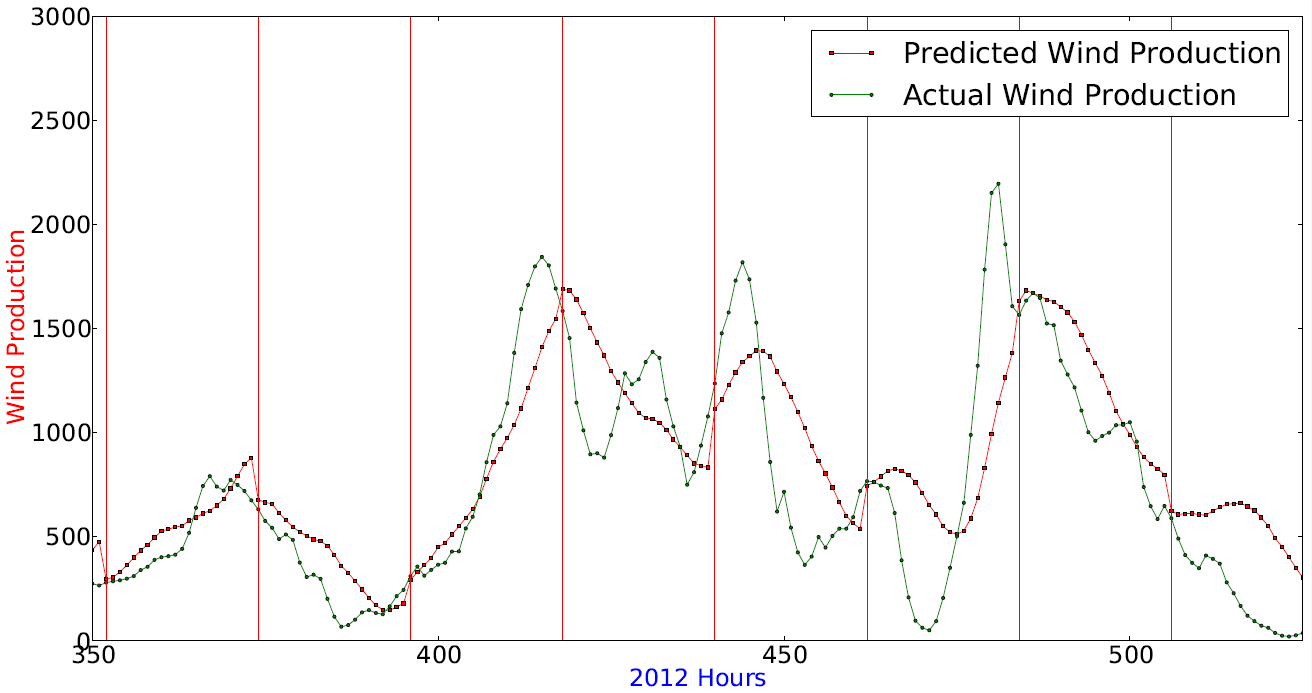
\includegraphics[width=0.99\linewidth]{billeder/best22vsbest24Ahead.png}
\caption{22-step-ahead forecast}
\label{fig:best22vsbest24Ahead}
\end{figure}

\begin{figure}[H]
\centering
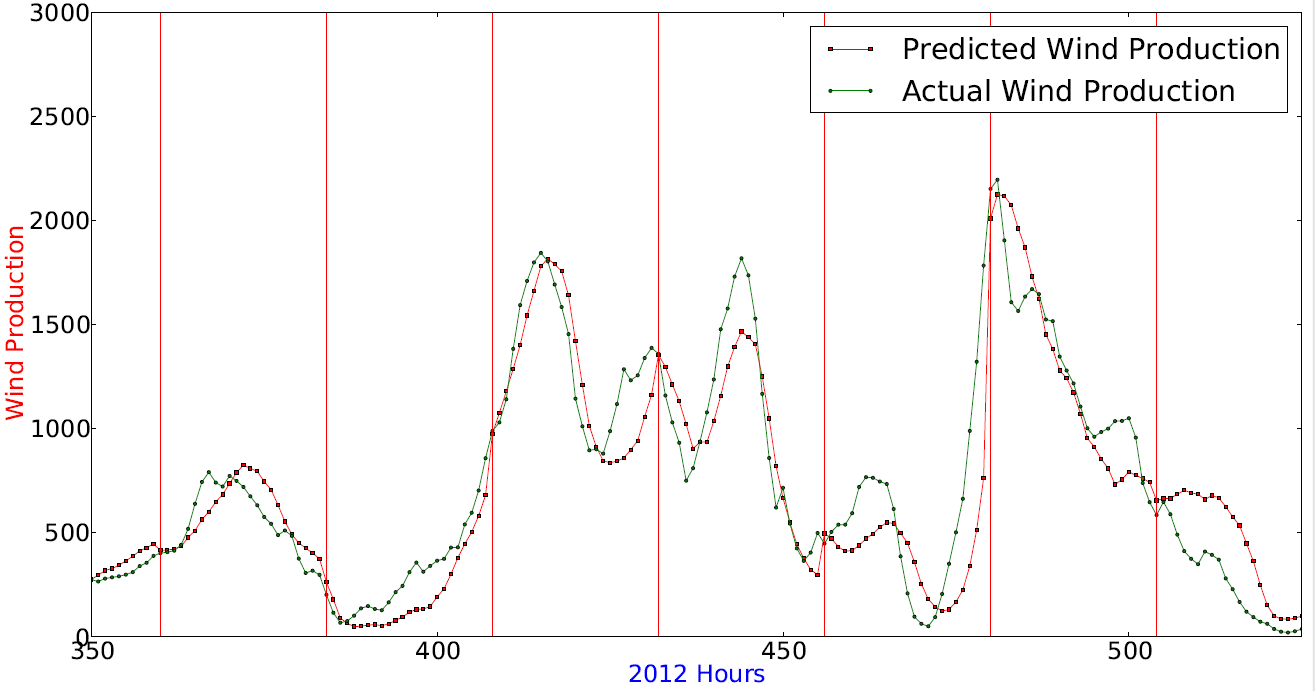
\includegraphics[width=0.99\linewidth]{billeder/best24AheadPredictionWithLines.png}
\caption{24-step-ahead forecast}
\label{fig:best24AheadPredictionWithLines}
\end{figure} 

\subsubsection{Offsets}
Due to the discussion regarding the different starting points (or offsets) we have performed experiments of them all to get an overview of the consequences to the error. All offsets have been tried in Table~\ref{table:stepAheadForecastingWindProductionStartingPositions} and it supports what was concluded from Table~\ref{table:stepAheadForecastingWindProduction}, e.g. that the offset greatly influence the result which must be considered by anyone using it. One thing that can possibly explain why offset 1 (which we have been using all along) achieves good results is the 24-hour cycle and how certain patterns apply from 00-24 every day of the year (the patterns are illustrated in Section~\ref{sec:greenTOD} and~\ref{sec:Price}). The position that has always been used is marked with an x. It is obvious here that the exact same prediction applied at various starting points differs much in accuracy. 

\begin{center}
\begin{longtable}{|c|c|c|c|c|}
\hline
\textbf{Steps ahead} & \textbf{MAPE} & \textbf{MAE} & \textbf{\% Deviation} & \textbf{\% Correct Direction} \\
\hline
\endfirsthead
\multicolumn{5}{c}%
{\tablename\ \thetable\ -- \textit{Continued from previous page}} \\
\hline
\textbf{Steps ahead} & \textbf{MAPE} & \textbf{MAE} & \textbf{\% Deviation} & \textbf{\% Correct Direction} \\
\hline
\endhead
\hline \multicolumn{5}{r}{\textit{Continued on next page}} \\
\endfoot
\endlastfoot
\arrayrulecolor{light-gray}
16 & 18,26\% & 121,73 & 0,0\% & 73\%  \\ \hline
1 (x) & 18,49\% & 122,84 & 0,9\% & 73\%  \\ \hline
8 & 18,61\% & 124,06 & 1,91\% & 72\%  \\ \hline
7 & 18,68\% & 124,52 & 2,29\% & 70\%  \\ \hline
14 & 18,92 & 126,12 & 3,67\% & 70\%  \\ \hline
13 & 19,12\% & 127,49 & 4,73\% & 70\%  \\ \hline
22 & 19,5\% & 129,94 & 6,74\% & 69\%  \\ \hline
17 & 19,58\% & 130,49 & 7,2\% & 70\%  \\ \hline
5 & 20,94\% & 139,56 & 14,65\% & 72\%  \\ \hline
24 & 20,97\% & 139,79 & 14,84\% & 72\%  \\ \hline
12 & 21,03\% & 140,15 & 15,13\% & 72\%  \\ \hline
3 & 21,04\% & 140,23 & 15,2\% & 72\%  \\ \hline
2 & 21,09\% & 140,57 & 15,48\% & 72\%  \\ \hline
19 & 21,1\% & 140,62 & 15,52\% & 72\%  \\ \hline
20 & 21,11\% & 140,68 & 15,57\% & 72\%  \\ \hline
10 & 21,13\% & 140,85 & 15,71\% & 72\%  \\ \hline
21 & 21,18\% & 141,19 & 15,99\% & 72\%  \\ \hline
18 & 21,19\% & 141,2 & 15,99\% & 72\%  \\ \hline
4 & 21,23\% & 141,51 & 16,25\% & 72\%  \\ \hline
23 & 21,31\% & 142,01 & 16,66\% & 72\%  \\ \hline
15 & 21,47\% & 143,08 & 17,54\% & 72\%  \\ \hline
11 & 21,57\% & 143,74 & 18,08\% & 72\%  \\ \hline
6 & 21,61\% & 144,04 & 18,33\% & 72\%  \\ \hline
9 & 22,71\% & 151,36 & 24,34\% & 71\%  \\ \hline
\caption{24-step-aheads forecast covering all starting positions}
\label{table:stepAheadForecastingWindProductionStartingPositions}
\end{longtable}
\end{center}





\todo{one step ahead vs. 24 ahead to show that is the same in the beginning on 24 timer}

\subsubsection{Conclusion}
The expectation was to see an improvement in MAE when predicting fewer hours which was seen in Table~\ref{table:stepAheadForecastingWindProduction}. It also showed that at some point the fewer hours is not necessarily better because they start at different positions and the prediction can correct itself the further it gets. The starting position has a huge impact on the accuracy of the prediction which was illustrated in the comparison between 22- and 24-step-ahead forecasts. It was further backed up by trying out all starting points with 24-step-ahead forecasting.

\subsection{Concluding Remarks}
Experiments have been conducted to identify the best combination of inputs as well as the impact of data manipulation, calculated inputs and black box optimization. Each experiment concludes on its findings in relation to experiments before it and expectations from the wind power production analysis. Table~\ref{table:comparisonOfResultsWindProduction} shows the overall improvement of 5,35\% from the first experiment to the last. Experiment five is left out in this table because it cannot be compared with the other since it predicts different number of hours. What have been observed throughout all experiments is the stable percentage of around 70\% in predicting the correct direction. It has also been discussed that the stability here lies in the co-relation to wind speed which is included as input in all experiments. The best result missed its target (in average) by 121 out of the interval from 0 to 2753 corresponding to 4,4\% of the 2753 potential values. We consider this to be satisfactory since it gives a clear indication of the wind power movements which was the purpose of the wind power prediction according to Section~\ref{sec:windPowerAnalysis}. 

\begin{enumerate}
\item First experiment showed the importance of the correct input parameters used in the Artificial Neural Network. Temperature, last known production, wind speed and time of day was the best combination. Air density and wind direction also showed themselves in top-3. Furthermore, too large datasets seriously decreased the accuracy due to over-training of the network.
\item Experiment two showed a slight increase (1,9\% in average improve for top-3) in accuracy when applying matrix on time of day. Trimming makes less sense in a prediction simulation for Wind Power since no completely irregular values exist in the wind power training set. The predictions with trimming showed a decrease in accuracy compared to without trimming because trimming ended up creating irregularities instead of removing them.
\item Third experiment tried different approaches to calculated inputs in relation to letting the network itself calculate statistics by adding various previous productions --- the approaches are slope calculation, skewness and volatility. The best of the approaches were volatility which obtained an increase of 3,52\% in relation to the prediction just without it.
\item The purpose of the fourth experiment was to identify the correct number of epochs and validate the correct size of the training set. The best size was 3 month of data and with 2-300 epochs. The experiment also illustrated how the network can easily be under- or overfitted with too many or few epochs, or be under- or overtrained  according to the size of the training set. The best prediction is considered to be in agreement with our purpose, namely to approach the wind power by applying different strategies and identifying what works and what does not.	
\item The fifth experiment regarding step-ahead forecasting illustrated how the error can be elevated due to how subsequent steps depend on the prediction from its predecessor. This experiment also uncovered the huge difference in starting points of the prediction. The results varied all the way from 121,73 to 151,36 in MAE. The best best configuration of input parameters, epochs and size of data is still considered to be the best since all experiments had the same starting point and therefore predicted the same hours in all steps. This will be discussed further.
\end{enumerate}

\footnotesize
\begin{center}
\begin{longtable}{|c|c|c|c|c|}
\hline
\textbf{Exp: 1} & \textbf{Exp: 2} & \textbf{Exp: 3} & \textbf{Exp: 4} & \textbf{Overall improvement} \\
\hline
\endfirsthead
\multicolumn{5}{c}%
{\tablename\ \thetable\ -- \textit{Continued from previous page}} \\
\hline
\textbf{Exp: 1} & \textbf{Exp: 2} & \textbf{Exp: 3} & \textbf{Exp: 4} & \textbf{Overall improvement} \\
\hline
\endhead
\hline \multicolumn{5}{r}{\textit{Continued on next page}} \\
\endfoot
\endlastfoot
\arrayrulecolor{light-gray}
128,32 &  126,25 & 121,81 & 121,02 & 5,7\% \\ \hline
\caption{Comparison of the best MAE from each of the experiment except from the fifth}
\label{table:comparisonOfResultsWindProduction}
\end{longtable}
\end{center}
\normalsize

\footnotesize
\begin{center}
\begin{longtable}{|c|c|c|c|c|}
\hline
\textbf{Exp: 1} & \textbf{Exp: 2} & \textbf{Exp: 3} & \textbf{Exp: 4} & \textbf{Overall improvement} \\
\hline
\endfirsthead
\multicolumn{5}{c}%
{\tablename\ \thetable\ -- \textit{Continued from previous page}} \\
\hline
\textbf{Exp: 1} & \textbf{Exp: 2} & \textbf{Exp: 3} & \textbf{Exp: 4} & \textbf{Overall improvement} \\
\hline
\endhead
\hline \multicolumn{5}{r}{\textit{Continued on next page}} \\
\endfoot
\endlastfoot
\arrayrulecolor{light-gray}
19,25\% &  18,94\% & 18,28\% & 18,16\% & 1,09\% \\ \hline
\caption{Comparison of the best MAPE from each of the experiment except from the fifth}
\label{table:comparisonOfResultsWindProduction}
\end{longtable}
\end{center}
\normalsize